% (c) 2012 Dimitrios Vrettos - d.vrettos@gmail.com
% (c) 2014 Claudio Carboncini - claudio.carboncini@gmail.com
% (c) 2014 Daniele Masini - d.masini.it@gmail.com
\chapter{Nozioni fondamentali}

\section{Introduzione alla geometria razionale}
\subsection{Breve nota storica}
La parola geometria deriva dal greco antico: \textgreek{gewmetr'ia}, composta da \textgreek{gew} (geo) che significa ``terra'' e da \textgreek{metr'ia} (metria) che significa ``misura'', tradotto alla lettera significa ``misura della terra''. Secondo una tradizione storica, durante il VI secolo \aC{} alcuni matematici e pensatori greci (principalmente Talete e Pitagora) cominciarono a organizzare in maniera razionale (secondo il susseguirsi di ragionamenti logici) le conoscenze geometriche che egiziani e babilonesi avevano raggiunto nei secoli precedenti. Lo storico greco Erodoto, vissuto tra il 484 \aC{} e il 425 \aC, racconta che a causa delle periodiche inondazioni del fiume Nilo gli egiziani erano costretti a ricostruire ogni anno i confini dei singoli possedimenti terrieri e in questo modo avevano sviluppato delle modalità tecniche per la misura della terra (\textgreek{gewmetr'ia} appunto).

Ritrovamenti più recenti di tavolette di creta del periodo babilonese incise con caratteri cuneiformi ci fanno ritenere che la cultura babilonese possedesse già delle sofisticate conoscenze geometriche. Di certo sappiamo che nel III secolo \aC{} il matematico ellenico Euclide\footnote{vissuto molto probabilmente durante il regno di Tolomeo I (367 \aC{} ca. - 283 \aC).}, direttore della grande biblioteca di Alessandria in Egitto, diede una struttura razionale alle conoscenze geometriche note sino ad allora scrivendo una delle più grandi opere della cultura occidentale, gli \emph{Elementi} (in greco \textgreek{Stoiqeia}). Questa grande opera è organizzata in 13 libri, di cui i primi sei riguardano la Geometria Piana, i successivi quattro trattano i rapporti tra grandezze e gli ultimi tre riguardano la Geometria Solida. Essa prese il posto di tutti i libri precedenti sulla geometria e servì come testo fondamentale nell'antichità e nel medioevo; è stata usata come libro scolastico di geometria fino ai nostri giorni. La sua considerazione presso i Romani fu modesta, ma fu grandissima presso i Bizantini e gli Arabi. Proprio questi ultimi la reintrodussero in Europa dopo la perdita medievale, grazie alla traduzione di Adelardo di Bath\footnote{traduttore, filosofo e matematico britannico (1080 - 1152).} (secolo XII).

Dal punto di vista della struttura logica, gli \emph{Elementi} di Euclide sono organizzati a partire da cinque assiomi (nozioni comuni evidenti), cinque postulati (proposizioni che si richiede siano assunte come vere, senza dimostrazione) e 23 definizioni. L'opera di Euclide è rimasta nella nostra cultura l'unico punto di riferimento per lo studio della geometria, fino a quando, contestualmente allo studio dei fondamenti delle altre branche della matematica, i matematici cercarono di dare una base più rigorosa alla geometria di Euclide. Un'impostazione assiomatica più moderna venne data dal matematico tedesco David Hilbert\footnote{(1862 - 1943).} nel libro \emph{Grundlagen der Geometrie} (Fondamenti della geometria) pubblicato nel 1899, nel quale la geometria veniva fondata su ben 21 assiomi.

\subsection{Lo spazio fisico e la geometria}
La geometria nasce come studio sistematico dello spazio fisico e delle forme che in esso si muovono. Lo spazio in cui ci muoviamo è per tutti una delle prime esperienze che facciamo fin dai primi mesi di vita. I nostri sensi determinano le sensazioni che ci permettono di riconoscere le forme degli oggetti e i loro movimenti. Tuttavia, le nozioni geometriche come quelle di punto, retta, rettangolo, cubo, sfera \ldots non trovano un perfetto riscontro nella realtà fisica. Nello spazio fisico non esistono, infatti, punti e rette come li descrive la geometria, né figure a due sole dimensioni, né cubi o sfere perfette. La geometria si propone quindi di fornire un ``modello'' ideale della realtà fisica, sia per le forme degli oggetti sia per le proprietà dello spazio. 

Fino alla seconda metà dell'Ottocento, matematici e filosofi sono stati sostanzialmente d'accordo nel considerare la geometria come la scienza che descriveva razionalmente le proprietà dello spazio fisico. Galileo ne \emph{Il saggiatore} (1623) scriveva:
\begin{quoting}
La filosofia è scritta in questo grandissimo libro che continuamente ci sta aperto innanzi a gli occhi (io dico l'universo), ma non si può intendere se prima non s'impara a intender la lingua, e conoscer i caratteri, ne' quali è scritto. Egli è scritto in lingua matematica, e i caratteri son triangoli, cerchi, ed altre figure geometriche, senza i quali mezi è impossibile a intenderne umanamente parola; senza questi è un aggirarsi vanamente per un oscuro laberinto.
\end{quoting}
A partire dalla seconda metà del XIX secolo, i matematici si sono invece convinti che la geometria non descrive esattamente lo spazio fisico, che sono possibili più geometrie ugualmente vere dal punto di vista logico e matematico. Lo studio matematico della geometria si è allora differenziato dallo studio dello spazio fisico e da quello dello spazio psicologico percepito dall'uomo con i suoi sensi. I matematici hanno accettato l'esistenza di diverse geometrie matematicamente possibili, si sono accontentati di costruire dei modelli astratti e hanno lasciato ai fisici la ``scelta'' del modello che meglio si adatta a descrivere i fenomeni fisici dall'infinitamente piccolo all'infinitamente grande. La geometria allora è diventata una branca della matematica alla quale i matematici hanno cercato di dare un fondamento esclusivamente logico, indipendente dalle esperienze fisiche. 

Il legame tra fisica e matematica non si è mai rotto. Con il passare dei secoli, ci si è resi sempre più conto di quanto la ``geometria'' del mondo fisico sia molto complessa e di come alcune nuove geometrie riescono a descrivere meglio fenomeni che con la vecchia geometria di Euclide non si riusciva a spiegare.

\section{Il metodo assiomatico, i concetti primitivi e le definizioni}
La geometria, sin dai tempi di Euclide, è stata organizzata assiomaticamente, partendo cioè dalle fondamenta. Nella matematica queste fondamenta sono costituite dai concetti primitivi e dagli assiomi. Gli \emph{enti primitivi} sono le nozioni che si decide di non definire. Ci si può rendere facilmente conto, infatti, che non tutto può essere definito, poiché in ogni nozione che si definisce si deve fare ricorso ad altre nozioni, le quali a loro volta devono essere definite per mezzo di altre nozioni e così via all'indietro senza che teoricamente questo processo abbia mai una fine, arrivando necessariamente ad alcune nozioni così primitive da non poter essere definite con altre nozioni più elementari. A queste nozioni non è né necessario né possibile associare alcun significato esplicito; è invece fondamentale esprimere le loro proprietà esclusivamente attraverso \emph{assiomi}, cioè attraverso proprietà non dimostrabili che indicano però come gli enti primitivi devono e possono essere usati. Il matematico Hilbert utilizza tre enti primitivi -- punto, linea e piano -- e 21 assiomi. A partire dagli enti primitivi si fanno derivare tutte le \emph{definizioni} degli enti geometrici.

\subsection{Nozioni di logica}

Assumiamo come ``primitivo'' il concetto base di proposizione (o ``giudizio'' secondo la terminologia del grande filosofo greco Aristotele\footnote{(384 o 383 \aC{} - 322 \aC).}): chiamiamo \emph{proposizione} una frase (affermativa o negativa) a cui abbia senso associare un valore di verità, sia esso \emph{vero} (V) oppure \emph{falso} (F).

Per esempio, sono proposizioni logiche affermazioni del tipo <<Una retta ha infiniti punti>>, <<$2+3=10$>>. Non sono proposizioni logiche le frasi <<\np{1000} è un numero grande>>, <<il quadrato è semplice>>. Mentre la prima frase esprime un'affermazione vera e la seconda un'affermazione falsa, la terza e la quarta esprimono affermazioni non valutabili oggettivamente pertanto di queste ultime non si può dire se sono vere o false.

La logica delle proposizioni si fonda sui seguenti tre principi della logica aristotelica:
\begin{itemize*}
\item il \emph{principio di identità}: ogni oggetto è identico a se stesso e a nessun altro oggetto;
\item il \emph{principio di non contraddizione}: una stessa proposizione non può essere contemporaneamente vera e falsa;
\item il \emph{principio del terzo escluso}: una proposizione può essere solo vera o falsa, non può assumere un diverso valore di verità.
\end{itemize*}

Il corpo della geometria, come di qualunque altra teoria matematica, è costituito da \emph{proposizioni}, cioè da affermazioni che riguardano gli enti geometrici e che sono vere o false. Le proposizioni possono essere semplici affermazioni (\emph{proposizioni atomiche}) oppure possono essere ottenute da una o più proposizioni elementari legate tra di loro attraverso connettivi logici (elementi linguistici del tipo ``non'', ``e'', ``oppure'', ``o \ldots{} o'', ``quindi'', ``se \ldots{} allora'', ``se e solo se''). In questo caso si parla di \emph{proposizioni composte} o molecolari
Per esempio, la proposizione <<un triangolo ha tre lati e ha tre angoli>> è composta dalle proposizioni <<un triangolo ha tre lati>> e <<un triangolo ha tre angoli>> unite dal connettivo ``e''.

\paragraph{La congiunzione} di due proposizioni si ottiene con il connettivo ``e'' (\emph{et}, \emph{and}, $\wedge$): la proposizione $r$ ottenuta dalla congiunzione delle proposizioni $p$ e $q$, in simboli può essere scritta come
\begin{empheq}[box=\fbox]{equation*}
\vphantom{I}r=p\wedge q
\end{empheq}
ed è vera se entrambe le proposizioni $p$ e $q$ sono contestualmente vere, mentre è falsa quando anche una sola delle due proposizioni è falsa.
Per esempio, <<ho avuto 7 in italiano e matematica>> è un'affermazione vera solo quando ho avuto 7 in entrambe le materie e falsa in tutti gli altri casi.

Per esprimere in maniera sintetica tutte le possibilità del valore di verità di una proposizione composta, si usa una tabella a doppia entrata, detta \emph{tavola di verità}, che per la congiunzione logica è la seguente
\begin{center}
 \begin{tabular*}{.25 \textwidth}{@{\extracolsep{\fill}}*{3}{c}}
 \toprule
~$p$ &~$q$ &~$p\wedge q$\\
\midrule
~V & V & V \\
~V & F & F \\
~F & V & F \\
~F & F & F \\
\bottomrule
 \end{tabular*}
\end{center}

\paragraph{La disgiunzione (inclusiva)} di due proposizioni si ottiene con il connettivo ``o'' (\emph{vel}, \emph{or}, ${\vee}$): la proposizione $s$ ottenuta dalla disgiunzione di due proposizioni $p$ e $q$, in simboli
\begin{empheq}[box=\fbox]{equation*}
\vphantom{I}s=p\vee q
\end{empheq}
è vera quando almeno una delle due proposizioni è vera ed è falsa solo se entrambe le proposizioni sono false.
\begin{center}
 \begin{tabular*}{.25 \textwidth}{@{\extracolsep{\fill}}*{3}{c}}
 \toprule
~$p$ &~$q$ &~$p\vee q$\\
\midrule
~V & V & V \\
~V & F & V \\
~F & V & V \\
~F & F & F \\
\bottomrule
 \end{tabular*}
\end{center}

\paragraph{La negazione} di una proposizione si ottiene con il connettivo ``non'' (\emph{non}, \emph{not}, $\neg$), un operatore che, a differenza dei precedenti, non lega più proposizioni ma agisce su un'unica proposizione (per questo si dice che è un operatore unario, in analogia all'operazione insiemistica di complementazione). La proposizione $n$ data dalla negazione di una proposizione $p$ si indica con il simbolo
\begin{empheq}[box=\fbox]{equation*}
\vphantom{I}n=\neg p
\end{empheq}
ed è vera se $p$ è falsa, viceversa è falsa se $p$ è vera.

La doppia negazione equivale ad un'affermazione, cioè $\neg(\neg p)$ è equivalente a $p$.
La tavola di verità è la seguente:
\begin{center}
 \begin{tabular*}{.25 \textwidth}{@{\extracolsep{\fill}}*{3}{c}}
 \toprule
~$p$ &~$\neg p$ &~$\neg(\neg p)$\\
\midrule
~V & F & V \\
~F & V & F \\
\bottomrule
 \end{tabular*}
\end{center}

\paragraph{La disgiunzione esclusiva} di due proposizioni si ottiene con il connettivo [o congiunzione] ``o \ldots{} o'' (\emph{aut}, \emph{xor}, $\veebar$): la proposizione $t$ ottenuta dalla disgiunzione esclusiva di due proposizioni $p$ e $q$, in simboli
\begin{empheq}[box=\fbox]{equation*}
\vphantom{I}t=p\veebar q
\end{empheq}
è vera quando solo una delle due proposizioni è vera ed è falsa quando le due proposizioni sono entrambe vere o entrambe false.
Per esempio, nell'affermazione <<oggi il Milan vince o pareggia>> la congiunzione ``o'' ha valore esclusivo.

La disgiunzione esclusiva $\veebar$ a volte non viene messa tra gli operatori logici fondamentali perché è esprimibile attraverso gli altri tre operatori presentati finora.
\begin{center}
 \begin{tabular*}{.25 \textwidth}{@{\extracolsep{\fill}}*{3}{c}}
 \toprule
~$p$ &~$q$ &~$p\veebar q$\\
\midrule
~V & V & F \\
~V & F & V \\
~F & V & V \\
~F & F & F \\
\bottomrule
 \end{tabular*}
\end{center}

\begin{exrig}
\begin{esempio}
Date le seguenti proposizioni $p=$~<<un triangolo ha tre lati>> (Vera), $q=$~<<un triangolo ha tre vertici>> (Vera), $r=$~<<un triangolo ha quattro angoli>> (Falsa), $s=$~<<un triangolo ha tre dimensioni>> (Falsa), allora:
\begin{itemize*}
\item $p\wedge q$ è vera,~~$q\wedge r$ è falsa,~~$r\wedge s$ è falsa;
\item $p\vee q$ è vera,~~$q\vee r$ è vera,~~$r\vee s$ è falsa;
\item $p\veebar q$ è falsa,~~$q\veebar r$ è vera,~~$r\veebar s$ è falsa.
\end{itemize*}
\end{esempio}
\end{exrig}

È piuttosto semplice capire il meccanismo della negazione se applicata a proposizioni atomiche, spesso è meno intuitivo il valore di verità della negazione di una proposizione più complessa.
Ad esempio, la negazione di $p\wedge q$ non è $\neg p\wedge \neg q$ bensì $\neg p\vee \neg q$, mentre la negazione di $p\vee q$ è $\neg p\wedge \neg q$ e non $\neg p\vee \neg q$.
In formule:
\begin{empheq}[box=\fbox]{equation*}
\vphantom{I}\neg (p\wedge q)= (\neg p)\vee (\neg q)\qquad\text{e}\qquad\neg (p\vee q)= (\neg p)\wedge (\neg q).
\end{empheq}

Per esempio, <<non è vero che Marco e Luca sono stati bocciati>> può voler dire che entrambi non sono stati bocciati o solo uno di loro non è stato bocciato.

Queste uguaglianze prendono il nome di \emph{leggi di De Morgan}\footnote{dal nome del matematico e logico britannico Augustuts De Morgan (1806 - 1871).}, e la loro verifica può essere effettuata con la seguente tavola di verità:
\begin{center}
 \begin{tabular*}{.8 \textwidth}{@{\extracolsep{\fill}}*{8}{c}}
 \toprule
~$p$ &~$q$ &~$ \neg p $&~$ \neg q $&~$p\wedge q$&~$\neg p\vee \neg q$&~$p\vee q$&~$\neg p\wedge \neg q$\\
\midrule
~V & V & F & F & V & F & V & F \\
~V & F & F & V & F & V & V & F \\
~F & V & V & F & V & V & V & F \\
~F & F & V & V & F & V & F & V \\
\bottomrule
 \end{tabular*}
\end{center}

Come per le operazioni aritmetiche anche per gli operatori logici è possibile analizzarne le proprietà. Ne indichiamo qualcuna a titolo di esempio:
\begin{itemize*}
\item $(p\wedge q)\wedge r= p\wedge (q\wedge r)$ proprietà \emph{associativa} della congiunzione;
\item $p\wedge q= q\wedge p$ proprietà \emph{commutativa} della congiunzione;
\item $p\wedge (q\vee r)= (p\wedge q)\vee (p\wedge r)$ proprietà \emph{distributiva} della congiunzione rispetto alla disgiunzione.
\end{itemize*}

Una proposizione che è sempre vera indipendentemente dalla verità degli elementi che lo compongono è detta \emph{tautologia}. Una proposizione che è sempre falsa indipendentemente dalla verità dei suoi elementi è invece detta \emph{contraddizione}.

Per esempio, la proposizione composta $p\wedge \neg p$ è una contraddizione in quanto è sempre falsa, mentre la proposizione composta $p\vee \neg p$ è una tautologia poiché è sempre vera.

\subsection{Predicati e quantificatori}

Una proposizione che fa riferimento a una proprietà o caratteristica di alcuni elementi di un insieme si chiama \emph{predicato} (o \emph{enunciato}). Le frasi formate da un predicato che ha alcuni argomenti incogniti si dicono \emph{enunciati aperti}.
Per esempio, $p=$~<<$x$ è un numero intero maggiore di 10>> è un enunciato aperto.

Consideriamo ora le seguenti affermazioni:
\begin{itemize*}
\item <<tutti gli uomini sono mortali>> si riferisce a un qualsiasi essere umano;
\item <<tutti i multipli di 6 sono anche multipli di 2>> è vera per tutti i numeri multipli di 6;
\item <<ogni numero negativo è minore di ogni numero positivo>>.
\end{itemize*}
I predicati precedenti non riguardano un elemento specifico ma una certa quantità di elementi. I termini ``tutti'' e ``ogni'', detti \emph{quantificatori universali}, indicano che una proprietà è vera per tutti gli elementi di un certo insieme. In logica matematica per indicare il quantificatore universale si usa il simbolo $\forall$, che si legge ``per ogni''.

Vediamo ora i seguenti predicati:
\begin{itemize*}
\item <<esiste un numero che elevato al quadrato dà $16$>>;
\item <<alcuni numeri pari sono anche multipli di $3$>>.
\end{itemize*}
Queste affermazioni esprimono proprietà che sono vere almeno per un elemento dell'insieme di riferimento: la prima frase è vera per i numeri $+4$ e $-4$, la seconda frase è vera per i numeri $6$, $12$, $18$, \ldots{}
I termini ``c'è almeno'', ``alcuni'', ``esiste almeno uno'' si dicono \emph{quantificatori esistenziali} ed in logica matematica si indicano con il simbolo $\exists$, che si legge ``esiste''.

Bisogna prestare particolare attenzione quando si negano frasi in cui compaiono i quantificatori. Per esempio la negazione di <<tutti i gatti fanno le fusa>> non è <<nessun gatto fa le fusa>> bensì <<non tutti i gatti fanno le fusa>> che si può esprimere anche con il quantificatore esistenziale <<C'è almeno un gatto che non fa le fusa>>.
La negazione della frase <<l'anno scorso siamo stati tutti promossi>> non è <<l'anno scorso siamo stati tutti bocciati>> ma <<l'anno scorso non siamo stati tutti promossi>> ovvero <<l'anno scorso c'è stato almeno uno di noi che non è stato promosso>>.
La negazione della proposizione $p=$~<<tutti i quadrati hanno due diagonali>> è la proposizione ${\lnot}p=$~<<non tutti i quadrati hanno due diagonali>>.
Il linguaggio comune ci potrebbe portare a considerare come negazione di $p$ la proposizione <<nessun quadrato ha due diagonali>>, in realtà per avere la negazione della proposizione $p$ basta che esista almeno un quadrato che non ha due diagonali.

\subsection{Implicazione}

Nel linguaggio matematico sono comuni proposizioni del tipo <<Se $p$ allora $q$>>. Ad esempio <<se un numero è multiplo di $12$ allora è multiplo di $3$>>. La frase precedente può essere espressa dicendo <<essere multiplo di $12$ \emph{implica} essere multiplo di $3$>>.

In logica frasi del tipo <<se $p$ allora $q$>> vengono tradotte utilizzando l'operatore $\Rightarrow$ detto \emph{implicazione}.
La scrittura <<se $p$ allora $q$>> si traduce quindi con la scrittura
\begin{empheq}[box=\fbox]{equation*}
\vphantom{I}p\Rightarrow q
\end{empheq}
che si legge ``$p$ implica $q$''.

La proposizione $p$ è detta \emph{antecedente}, (o \emph{ipotesi}) e la proposizione $q$ è detta \emph{conseguente} (o \emph{tesi}).
Il significato logico della proposizione $p\Rightarrow q$ è che <<tutte le volte che la proposizione $p$ è vera allora risulta vera anche la proposizione $q$>>. Ovvero non si specifica il caso in cui $p$ sia falsa.

Per esempio, l'affermazione <<se c'è il sole andiamo al mare>> è falsa solo quando c'è il sole e non andiamo al mare; l'affermazione, infatti, non dice nulla se il sole non c'è: quindi se non c'è il sole si è liberi di andare o non andare al mare. Anche l'affermazione <<se studi sarai promosso>> dice solo che se studi conseguirai la promozione, non dice nulla per il caso in cui tu non studi: in questo caso, infatti, potresti essere ugualmente promosso.

La tavola di verità è la seguente:
\begin{center}
 \begin{tabular*}{.25 \textwidth}{@{\extracolsep{\fill}}*{3}{c}}
 \toprule
~$p$ &~$q$ &~$p\Rightarrow q$\\
\midrule
~V & V & V \\
~V & F & F \\
~F & V & V \\
~F & F & V \\
\bottomrule
 \end{tabular*}
\end{center}

Uno degli errori logici più comuni è quello di pensare che da $p\Rightarrow q$ si possa dedurre  $\neg p\Rightarrow \neg q$.
Ad esempio dall'affermazione <<se piove prendo l'ombrello>> qualcuno può pensare che si possa dedurre <<se non piove non prendo l'ombrello>>. Riflettendoci, si intuisce che le due frasi non sono affatto consequenziali. Basta pensare che chi pronuncia la prima frase sta affermando che tutte le volte che piove prende naturalmente l'ombrello, ma non esclude la possibilità di prenderlo anche quando non piove (in effetti è saggio farlo se il cielo è coperto da nuvoloni neri!).

Così la frase (a) <<se $x$ è multiplo di $12$ allora è multiplo di $3$>> non vuol dire (b) <<se $x$ non è multiplo di $12$ allora non è multiplo di $3$>>.
Infatti la (a) è vera, mentre la (b) è falsa (si pensi ad esempio al numero $6$ che non è multiplo di $12$ ma è comunque multiplo di $3$).

Ciò che ragionevolmente si può dedurre da $p\Rightarrow q$ è $\neg q\Rightarrow \neg p$.
Ad esempio, da <<se $x$ è multiplo di $12$ allora è multiplo di $3$>> si può dedurre <<se $x$ non è multiplo di $3$ allora non è multiplo di $12$>>.

Data l'implicazione $p\Rightarrow q$, la proposizione $p$ viene detta \emph{condizione sufficiente} per $q$. Mentre la proposizione $q$ viene detta \emph{condizione necessaria} per $p$.
Per esempio, <<studiare>> è condizione necessaria per <<essere promossi>> ma non è sufficiente.
Quest'ultima espressione fa appunto riferimento al fatto che da $p\Rightarrow q$ si può dedurre  $\neg q\Rightarrow \neg p$. Ossia $q$ è necessaria per $p$ in quanto se non è vera $q$ non è vera neanche $p$.

Calcoliamo la tavola di verità di $p\Rightarrow q$ e di $\neg q\Rightarrow \neg p$ 
\begin{center}
 \begin{tabular*}{.6 \textwidth}{@{\extracolsep{\fill}}*{6}{c}}
 \toprule
~$p$ &~$q$ &~$p\Rightarrow q$ &~$ \neg q $ &~$ \neg p $&~$ \neg q\Rightarrow \neg p $ \\
\midrule
~V & V & V & F & F & V\\
~V & F & F & V & F & F\\
~F & V & V & F & V & V\\
~F & F & V & V & V & V\\
\bottomrule
 \end{tabular*}
\end{center}
Come si vede, le due proposizioni hanno gli stessi valori di verità.

In generale, data un'implicazione $p\Rightarrow q$ (\emph{proposizione diretta}):
\begin{itemize*}
\item l'implicazione $\neg p\Rightarrow \neg q$ si dice \emph{contraria} di $p\Rightarrow q$;
\item l'implicazione $q\Rightarrow p$ si dice \emph{inversa} di $p\Rightarrow q$;
\item l'implicazione $\neg q\Rightarrow \neg p$ si dice \emph{contronominale} (o \emph{controinversa}) di $p\Rightarrow q$.
\end{itemize*}

\paragraph{La doppia implicazione} o \emph{equivalenza logica} di due proposizioni $p$ e $q$ dà luogo a una proposizione che in simboli si rappresenta con
\begin{empheq}[box=\fbox]{equation*}
\vphantom{I}p\Leftrightarrow q
\end{empheq}
(leggasi ``$p$ se e solo se $q$'') che è vera solo se $p$ e $q$ sono entrambe vere o entrambe false. La tavola di verità è la seguente:
\begin{center}
 \begin{tabular*}{.75 \textwidth}{@{\extracolsep{\fill}}*{6}{c}}
 \toprule
~$p$ &~$q$ &~$p\Leftrightarrow q$ &~$ p\Rightarrow q $ &~$ q\Rightarrow p $&~$ (p\Rightarrow q)\wedge (q\Rightarrow p) $ \\
\midrule
~V & V & V & V & V & V\\
~V & F & F & F & V & F\\
~F & V & F & V & F & F\\
~F & F & V & V & V & V\\
\bottomrule
 \end{tabular*}
\end{center}
L'operatore $\Leftrightarrow $ è detto \emph{doppia implicazione} perché se vale $p\Leftrightarrow q$ allora valgono sia $p\Rightarrow q$ che $q\Rightarrow p$ (e viceversa). Nella tabella precedente, infatti, è stata messa in evidenza l'equivalenza logica tra la proposizione $p\Leftrightarrow q$ e la proposizione $(p\Rightarrow q)\wedge (q\Rightarrow p)$.

L'equivalenza logica è un relazione di equivalenza, infatti verifica le seguenti proprietà:
\begin{itemize*}
\item $p\Leftrightarrow p$: è \emph{riflessiva};
\item se $p\Leftrightarrow q$ allora vale anche $q\Leftrightarrow p$: è \emph{simmetrica};
\item se $p\Leftrightarrow q$ e $q\Leftrightarrow r$ allora vale anche $p\Leftrightarrow r$: è \emph{transitiva}.
\end{itemize*}

In matematica si usa spesso l'espressione <<$p$ è \emph{condizione necessaria e sufficiente} per $q$>>. Per esempio <<condizione necessaria e sufficiente affinché un numero sia divisibile per $3$ è che la somma delle sue cifre sia divisibile per $3$>>. Il significato della frase è che <<$p$ è sufficiente per $q$>> e inoltre <<$p$ è necessario per $q$>>. In altre parole significa che  $p\Rightarrow q$ e $q\Rightarrow p$. Nel caso dell'esempio vale quindi sia l'implicazione diretta, <<se un numero è divisibile per $3$ allora la somma delle sue cifre è divisibile per $3$>>, che quella inversa, <<se la somma delle cifre di un numero è divisibile per $3$ allora il numero stesso è divisibile per $3$>>.

\subsection{I teoremi}

Un \emph{teorema} è una proposizione composta del tipo  $I\Rightarrow T$, cioè una implicazione tra due proposizioni, dette \emph{ipotesi} ($I$) e \emph{tesi} ($T$).

Dimostrare un teorema significa fare un ragionamento logico che permetta di concludere che la tesi è vera avendo supposto che l'ipotesi sia vera. Nel caso in cui un teorema sia dimostrabile all'interno di una teoria, si dice che è un teorema valido.

In riferimento alla terminologia usata quando abbiamo parlato dell'implicazione, chiamiamo  $I\Rightarrow T$ \emph{teorema diretto}, $T\Rightarrow I$ \emph{teorema inverso}, $\neg I\Rightarrow \neg T$ \emph{teorema contrario} e $\neg T\Rightarrow \neg I$ \emph{teorema controinverso}. Ribadiamo l'equivalenza tra il teorema diretto ed il teorema controinverso, nonché l'equivalenza tra il teorema contrario ed il teorema inverso, mentre in generale la validità del teorema diretto non implica la validità del teorema inverso, e viceversa.

Nel caso particolare in cui vale sia $I\Rightarrow T$ che $T\Rightarrow I$, si scrive  $I\Leftrightarrow T$ e si dice che ipotesi e tesi sono \emph{logicamente equivalenti}. Più precisamente, nel linguaggio specifico delle scienze che fanno uso della logica, e quindi anche nel linguaggio della Geometria Razionale, se vale $I\Rightarrow T$, si dice che <<$I$ è condizione sufficiente per $T$>> e anche che <<$T$ è condizione necessaria per $I$>>; se in particolare vale  $I\Leftrightarrow T$, si usa dire che <<$I$ è condizione necessaria e sufficiente per $T$>>.

In generale incontreremo molti teoremi che vengono denominati genericamente \emph{proposizioni}, perché il nome di ``teorema'' viene tradizionalmente attribuito solo ai teoremi più importanti. Inoltre si usa chiamare \emph{lemma} una proposizione che non ha una grande importanza di per sé, ma che è particolarmente utile per la dimostrazione di altri teoremi. Si chiama invece \emph{corollario} un teorema importante che è una conseguenza immediata di un altro teorema.

Così come abbiamo visto che non è possibile definire tutto e che quindi bisogna assumere alcune nozioni come primitive, analogamente non è possibile dimostrare tutte le proposizioni di una teoria. Alcune proposizioni devono essere assunte come vere e costituiscono la base della dimostrazione dei teoremi; queste proposizioni si chiamano \emph{postulati} o \emph{assiomi}. Risulta evidente che cambiando sia pure uno solo degli assiomi cambiano anche i teoremi dimostrabili e quindi la teoria.

In generale, come abbiamo detto, dato un teorema (diretto) del tipo $p\Rightarrow q$, la sua validità non garantisce la validità del teorema inverso $q\Rightarrow p$. Questo però può succedere. In ogni caso, se sono vere $p\Rightarrow q$ e $q\Rightarrow p$, le due proposizioni sono \emph{logicamente equivalenti}, ossia $p\Leftrightarrow q$.
\begin{exrig}
\begin{esempio}
Teorema: <<un triangolo che ha i lati uguali ha anche gli angoli uguali>>.
\begin{itemize}
\item Il teorema si può schematizzare nel seguente modo: $p=$~<<un triangolo ha i lati uguali>>; $q=$~<<un triangolo ha gli angoli uguali>>. Il teorema enunciato è $p\Rightarrow q$.
\item  Il teorema inverso è  $q\Rightarrow p$, cioè <<un triangolo che ha gli angoli uguali ha anche i lati uguali>>.
\end{itemize}
In tale esempio sono validi sia il teorema diretto che quello inverso. Il fatto che uno dei due teoremi sia chiamato diretto e l'altro inverso è un fatto soggettivo, che può dipendere semplicemente dall'ordine con cui si enunciano i teoremi.
Il teorema precedente si può esporre allora nel seguente modo:
\item Teorema: <<un triangolo ha i lati uguali se e solo se ha gli angoli uguali>>.
\end{esempio}
\end{exrig}

\subsection{La deduzione}

Nel paragrafo precedente abbiamo parlato in modo generico di implicazione, deduzione, dimostrazione. Facciamo ora un po' di chiarezza sull'uso di questi termini. L'\emph{implicazione} è un'operazione tra proposizioni, mentre la \emph{deduzione} è il ragionamento logico che costituisce la base della dimostrazione di un teorema. Per l'implicazione materiale si usa il simbolo $\rightarrow$ mentre per la deduzione logica si usa il simbolo $\Rightarrow$.

La frase <<se 5 è un numero pari, allora il triangolo ha 4 lati>> è perfettamente valida dal punto di vista logico ed anzi è vera, poiché la premessa (proposizione antecedente) è falsa, per cui l'implicazione è vera anche se la proposizione conseguente è falsa (si tenga presente la tavola di verità di $p\Rightarrow q$).
Si noti però che la definizione di implicazione ha senso solamente se la premessa è vera, il suo ampliamento al caso in cui la premessa è falsa è motivata da ragioni di completezza della trattazione. Bisogna quindi fare attenzione ad usare l'implicazione logica quando la premessa è falsa. Teniamo comunque conto che se $p$ è falsa allora $(p\Rightarrow q)\wedge(p\Rightarrow \neg q)$ cioè $p\Rightarrow (q\wedge \neg q)$ è vera. Ma  $q\wedge \neg q$ è una contraddizione, quindi una premessa falsa implica sempre una contraddizione.

In realtà, la \emph{dimostrazione} di un teorema non è la verifica della validità dell'implicazione, anzi è un procedimento che fa uso della validità dell'implicazione stessa. In un teorema si parte dal supporre vera l'ipotesi e si dimostra, mediante un ragionamento logico che si basa sugli assiomi e su altri teoremi già dimostrati in precedenza, che anche la tesi è vera (questo se si segue il \emph{procedimento diretto}). Se si segue invece il \emph{procedimento indiretto} (o \emph{per assurdo}), si suppone che la tesi sia falsa e, sempre mediante ragionamento logico basato su assiomi e altri teoremi già dimostrati, si arriva ad affermare che l'ipotesi è falsa (cosa che non si deve accettare).

Le principali regole del corretto ragionamento seguono alcuni schemi particolari (detti \emph{sillogismi}, dal nome attribuito ad essi da Aristotele). Presentiamo qui i quattro principali sillogismi: il \emph{modus ponens}, il \emph{modus tollens}, il \emph{sillogismo disgiuntivo} e il \emph{sillogismo ipotetico}.
\begin{center}
 \begin{tabular*}{.8 \textwidth}{@{\extracolsep{\fill}}*{6}{c}}
 \toprule
 &Modus&Modus&\multicolumn{2}{c}{Sillogismo}&Sillogismo\\
 &ponens&tollens&\multicolumn{2}{c}{disgiuntivo}&ipotetico\\
\midrule
1\textsuperscript{a} premessa & $p\Rightarrow q$ & $p\Rightarrow q$ & $p\vee q$ & $p\vee q$ & $p\Rightarrow q$\\
2\textsuperscript{a} premessa & $ p $ & $ \neg q $ & $ \neg p $ & $ \neg q $  & $q\Rightarrow r$\\
\midrule
conclusione & $ q $ & $ \neg p $ & $ q $ & $ p $ & $p\Rightarrow r$\\
\bottomrule
 \end{tabular*}
\end{center}
Suggeriamo una lettura degli schemi appena esposti:
\begin{itemize}
\item \emph{modus ponens}: se sappiamo che $p$ implica $q$ e che $p$ è vera, allora possiamo concludere che anche $q$ è vera (metodo diretto di dimostrazione);
\item \emph{modus tollens}: se sappiamo che $p$ implica $q$ e che $q$ è falsa, allora possiamo concludere che anche $p$ è falsa (metodo indiretto di dimostrazione);
\item \emph{sillogismo disgiuntivo}: se sappiamo che, tra $p$ e $q$, almeno una delle due è vera, e sappiamo che $p$ (rispettivamente $q$) è falsa, allora possiamo concludere che $q$ (rispettivamente $p$) è vera;
\item \emph{sillogismo ipotetico}: se sappiamo che $p$ implica $q$ e che $q$ implica $r$, allora possiamo concludere che $p$ implica $r$ (proprietà transitiva dell'implicazione).
\end{itemize}

Altre regole (note come i \emph{giudizi} di Aristotele) fanno uso dei predicati e dei quantificatori. Riprendiamo un esempio precedente traducendo la frase <<tutti i quadrati hanno due diagonali>> e la sua negazione <<non tutti i quadrati hanno due diagonali>> in formule che fanno uso anche del linguaggio degli insiemi. Se chiamiamo $Q$ l'insieme di tutti i quadrati e $P$ la proprietà dell'avere due diagonali, se $x$ è il generico quadrato (elemento di $Q$), $P(x)$ è il predicato <<$x$ gode della proprietà $P$>>, cioè <<$x$ ha due diagonali>>, la frase <<tutti i quadrati hanno due diagonali>> si traduce in simboli: ${\forall}x\in Q$, $P(x)$.

La sua negazione è: <<esiste almeno un quadrato che non ha due diagonali>>, cioè che non gode della proprietà $P$, e si traduce in simboli così: $\exists x\in Q$, $\neg P(x)$.
In quest'ultimo caso, la virgola può anche essere sostituita da una barra verticale (``\textbar'') o da ``:'' e si legge ``tale che''.

Analogamente, una frase del tipo <<esiste almeno un numero naturale che sia divisore di $10$>> può scriversi come: $\exists n\in\insN\mid D(n)$, dove $D$ è la proprietà dell'essere divisore di $10$ e $D(n)$ significa che $n$ verifica la proprietà $D$, cioè che $n$ è un divisore di $10$. La sua negazione è <<nessun numero naturale è divisore di 10>>, ovvero <<preso un qualsiasi numero naturale $n$, questo non gode della proprietà $D$>>, la traduzione in simboli di tale frase è: $\forall n\in\insN$, ${\neg}D(n)$.

Mettiamo in tabella le quattro proposizioni, che corrispondono ai giudizi di Aristotele):
%\begin{center}
% \begin{tabular*}{.8 \textwidth}{@{\extracolsep{\fill}}*{2}{l}}
% \multirow{2}*{A: Giudizio universale affermativo}&$\forall x\in Q$, $P(x)$\\
% & $P$ è vera per ogni $x$ \\
%\midrule
% \multirow{2}*{E: Giudizio universale negativo}&$\forall n\in\insN$, $\neg D(n)$\\
% & $D$ è falsa per ogni $n$ \\
%\midrule
% \multirow{2}*{I: Giudizio particolare positivo}&$\exists n\in\insN\mid D(n)$\\
% & $D$ è vera per almeno un $n$ \\
%\midrule
% \multirow{2}*{O: Giudizio particolare negativo}&$\exists x\in Q\mid\neg P(x)$\\
% & $P$ è falsa per almeno un $x$ \\
% \end{tabular*}
%\end{center}
\begin{center}
 \begin{tabular}{cc|cc}
 \toprule
 \multirow{3}{2.5cm}{A: Giudizio universale affermativo}&$\forall x\in Q$, $P(x)$&\multirow{3}{2.5cm}{I: Giudizio particolare affermativo}&$\exists n\in\insN\mid D(n)$\\
&\multirow{2}*{$P$ è vera per ogni $x$}& &\multirow{2}*{$D$ è vera per almeno un $n$}\\
&&&\\
\midrule
 \multirow{3}{2.5cm}{E: Giudizio universale negativo}&$\forall n\in\insN$, $\neg D(n)$&\multirow{3}{2.5cm}{O: Giudizio particolare negativo}&$\exists x\in Q\mid\neg P(x)$\\
 &\multirow{2}*{$D$ è falsa per ogni $n$}& &\multirow{2}*{$P$ è falsa per almeno un $x$}\\
 &&&\\
 \bottomrule
 \end{tabular}
\end{center}
I quattro giudizi di Aristotele si possono rappresentare con gli insiemi di Venn (figura~\ref{fig:1.1}).
\begin{figure}[bth]
 \centering% (c) 2014 Daniele Masini - d.masini.it@gmail.com
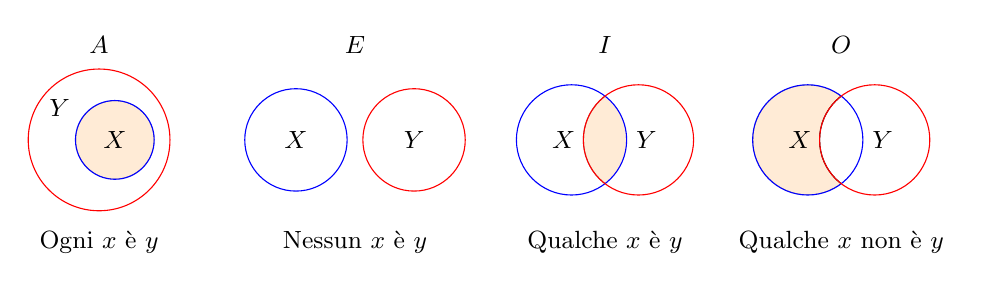
\begin{tikzpicture}[scale=1,font=\small]
\usetikzlibrary{calc}


\begin{scope}
\coordinate (oy) at (0,0);
\coordinate (ox) at (.2,0);
\draw[red] (oy) circle (0.9);

\begin{scope}
\clip (ox) circle (0.5);
\draw[fill=orange!40,opacity=.4] (ox) circle (0.5);
\end{scope}

\draw[blue] (ox) circle (.5);
\node at(.2,0){$X$};
\node at(-.5,.4){$Y$};
\node at(0,1.2){$A$};
\node at(0,-1.3){Ogni $x$ è $y$};
\end{scope}

\begin{scope}[xshift=2.5cm]
\coordinate (ox) at (0,0);
\coordinate (oy) at (1.5,0);
\draw[blue] (ox) circle (0.65);
\draw[red] (oy) circle (0.65);
\node at(0,0){$X$};
\node at(1.5,0){$Y$};
\node at(0.75,1.2){$E$};
\node at(0.75,-1.3){Nessun $x$ è $y$};
\end{scope}

\begin{scope}[xshift=6cm]
\coordinate (ox) at (0,0);
\coordinate (oy) at (0.85,0);

\begin{scope}
\clip (ox) circle (0.7);
\draw[fill=orange!40,opacity=.4] (oy) circle (0.7);
\end{scope}

\draw[blue] (ox) circle (0.7);
\draw[red] (oy) circle (0.7);

\node at(-0.1,0){$X$};
\node at(0.95,0){$Y$};
\node at(0.425,1.2){$I$};
\node at(0.425,-1.3){Qualche $x$ è $y$};
\end{scope}

\begin{scope}[xshift=9cm]
\coordinate (ox) at (0,0);
\coordinate (oy) at (0.85,0);

\begin{scope}
\clip (ox) circle (0.7);
\draw[fill=orange!40,opacity=.4] (ox) circle (0.7);
\draw[fill=white] (oy) circle (0.7);
\end{scope}

\draw[blue] (ox) circle (0.7);
\draw[red] (oy) circle (0.7);

\node at(-0.1,0){$X$};
\node at(0.95,0){$Y$};
\node at(0.425,1.2){$O$};
\node at(0.425,-1.3){Qualche $x$ non è $y$};
\end{scope}



\end{tikzpicture}
 \caption{Rappresentazione con gli insiemi di Venn dei giudizi di Aristotele}\label{fig:1.1}
\end{figure}

\subsection{La dimostrazione}

Tenendo conto di quanto detto precedentemente, dimostrare che $I\Rightarrow T$ significa fare un ragionamento logico che permetta di concludere che la tesi $T$ è vera avendo supposto che l'ipotesi $I$ sia vera.

Quando attraverso un ragionamento logico, e cioè attraverso una catena di implicazioni del tipo  $I\Rightarrow A\Rightarrow B\Rightarrow \ldots{} \Rightarrow T$, si riesce a dedurre la verità di una proposizione $T$ a partire dalla verità di una proposizione $I$. Si dice che si è data una \emph{dimostrazione diretta} del teorema $I\Rightarrow T$ (attraverso le regole del modus ponens e del sillogismo ipotetico).

Un teorema può anche essere \emph{dimostrato per assurdo}, o con metodo \emph{indiretto}. Questo tipo di dimostrazione consiste nel partire dalla negazione di $T$ e, attraverso una catena di implicazioni, arrivare alla negazione di $I$ o, in generale, ad una contraddizione.

Esistono altri metodi di dimostrazione, di cui eventualmente si parlerà più diffusamente qualora si dovesse ricorrere ad essi. Per ora ci limitiamo a citarne un paio: \emph{dimostrazione per induzione} e \emph{dimostrazione mediante esempio} o \emph{controesempio}.

La \emph{dimostrazione per induzione} si usa in particolare quando vogliamo dimostrare una proprietà generale che vale per molte categorie di figure ma che non si può esprimere in maniera unica per tutte le categorie (ad esempio una proprietà che vale per tutti i poligoni ma che dipende dal numero dei lati, come l'estensione dei criteri di congruenza dei triangoli a poligoni di più lati).

Si usa invece un \emph{esempio} quando bisogna dimostrare che una certa proprietà vale per almeno un oggetto del nostro studio o un \emph{controesempio} per dimostrare che una proprietà non vale per tutti gli oggetti in esame.

Per fornire alcuni esempi di dimostrazione, avremmo bisogno di fissare prima i concetti di base e gli assiomi da cui partire, per cui rinviamo la questione al prossimo paragrafo.

Ma a cosa serve studiare la dimostrazione di un teorema? Perché non ci limitiamo ad elencare i teoremi? Per molte applicazioni basta in effetti conoscere il teorema e a volte anche soltanto la formula risolutiva. Tuttavia studiando le dimostrazioni si impara a dimostrare e quindi si impara a creare nuova matematica. Un altro importante vantaggio è che la dimostrazione spiega perché il teorema è vero e permette di scoprire la struttura nascosta nelle definizioni e nei teoremi.

Quando si studia una dimostrazione non bisogna limitarsi a leggerla e a impararla a memoria, occorre leggerla attivamente, ponendo attenzione su cosa si fa e cercando di anticipare i passaggi. Se un passaggio non è chiaro bisogna prima tornare indietro per capire come ci si è arrivati e quindi cercare di capire il motivo per cui l'autore ha messo quel passaggio. In generale, una dimostrazione va letta più volte smettendo solo quando la si è compresa a fondo.


\section{Gli enti fondamentali della geometria}

In questo paragrafo diamo un cenno del sistema assiomatico della geometria razionale facendo riferimento principalmente all'impostazione assiomatica di Hilbert.

\subsection{Concetti primitivi}

Sono concetti primitivi per la geometria il \emph{punto}, la \emph{retta} e il \emph{piano}. Di essi non si dà una definizione e costituiscono la base per definire tutti gli altri enti della geometria.

Oltre a questi tre enti primitivi occorre poi assumere l'esistenza di tre relazioni primitive tra gli enti geometrici: \emph{giacere su}, \emph{stare fra}, \emph{essere congruente a}. Queste relazioni permettono di stabilire dei legami tra gli enti geometrici, per esempio: <<un punto giace su una retta>>, <<un punto sta fra altri due punti>>, <<un segmento è congruente a un altro segmento>>, \ldots

Esiste una simbologia convenzionale, condivisa dagli studiosi, per indicare questi enti:
\begin{itemize}
\item per indicare un punto usiamo una lettera maiuscola: $A$, $B$, $C$, \ldots;
\item per indicare una retta usiamo una lettera minuscola: $a$, $b$, $c$, \ldots;
\item per indicare un piano usiamo una lettera greca: $\alpha$, $\beta$, $\gamma$, \ldots
\end{itemize}

Ricordiamo l'alfabeto greco:
\begin{itemize}
\item lettere greche minuscole:  $\alpha$~(alfa),  $\beta$~(beta),  $\gamma$~(gamma),  $\delta$~(delta), $\epsilon$~(epsilon), $\zeta$~(zeta), $\eta$~(eta), $\theta$~(theta),  $\iota$~(iota),  $\kappa$~(kappa), $\lambda$~(lambda), $\mu$~(mi), $\nu$~(ni),  $\xi$~(xi), $o$~(omicron), $\pi$~(pi~o~pi~greca), $\rho$~(rho), $\sigma$~(sigma), $\tau$~(tau), $\upsilon$~(ipsilon), $\phi$~(fi), $\chi$~(chi), $\psi$~(psi), $\omega$~(omega);
\item lettere greche maiuscole: $A$, $B$, $ \Gamma $, $ \Delta $, $ E $, $ Z $, $ H $, $ \Theta $, $ I $, $ K $, $ \Lambda $, $ M $, $ N $, $ \Xi $, $ O $, $ \Pi $, $ \Sigma $, $ T $, $ \Upsilon $, $ \Phi $, $ X $, $ \Psi $, $\Omega $.
\end{itemize}

Degli enti fondamentali Euclide aveva dato le seguenti definizioni:
\begin{itemize*}
\item \emph{punto} è ciò che non ha parti;
\item \emph{linea} è lunghezza senza larghezza;
\item \emph{superficie piana} è quella che giace ugualmente rispetto alle rette su di essa.
\end{itemize*}
Le definizioni in questo caso sono utili per farci un'idea intuitiva degli enti stessi. Tuttavia, come è già stato detto in precedenza, e da quanto si intuisce osservando le definizioni euclidee, per definire il punto si utilizza la nozione di parte: ``punto è ciò che non ha parti''. Occorrerebbe quindi definire che cosa è una ``parte''. Ma per definire un parte avremmo bisogno di altre nozioni di partenza, in un procedimento senza fine. Per questo motivo nell'impostazione assiomatica moderna si preferisce non dare la definizione dei tre enti primitivi e ``definirli implicitamente'' attraverso le proprietà di cui godono. Ciò significa che si preferisce dare maggiore importanza a come essi si comportano e cosa possiamo fare con essi, piuttosto che descrivere cosa sono.
Dal punto di vista della rappresentazione grafica si usano le convenzioni come nella figura~\ref{fig:1.2}:
%\begin{center}
% \begin{tikzpicture}[font=\small]
%i punti
\tkzDefPoint(0,0){A}
\tkzDefPoint(1.5,1){B}
\tkzDefPoint(1,-1){C}
\tkzDrawPoints(A,B,C)
\tkzLabelPoints(A,B,C)
\node at(.75,-2){punti};

%le rette
\tkzDefPoint(3,-.5){D}
\tkzDefShiftPoint[D](30:1){E}
\tkzDefShiftPoint[D](30:3){F}
\tkzDefShiftPoint[D](30:4){G}
\tkzDrawSegments[style=dashed](D,E F,G)
\tkzDrawSegment(E,F)
\node at(4.3,.5){r};
\node at(4.3,-.5){s};

\tkzDefPoint(3,-1){D}
\tkzDefShiftPoint[D](35:1){E}
\tkzDefShiftPoint[D](35:3){F}
\tkzDefShiftPoint[D](35:4){G}
\tkzDrawSegments[style=dashed](D,E F,G)
\tkzDrawSegment(E,F)
\node at(4,-1-1){rette};

%il piano
\tkzDefPoint(6,-1){H}
\tkzDefShiftPoint[H](60:2.5){I}
\tkzDefShiftPoint[I](0:3){L}
\tkzDefShiftPoint[H](0:3){M}
\tkzDrawPolygon[fill=blue!10](H,I,L,M)
\node at(7.5,-1-1){piano};
\node at(10.3,.7){$\pi$};

\end{tikzpicture}

%\end{center}
\begin{figure}[htb]
 \centering\begin{tikzpicture}[font=\small]
%i punti
\tkzDefPoint(0,0){A}
\tkzDefPoint(1.5,1){B}
\tkzDefPoint(1,-1){C}
\tkzDrawPoints(A,B,C)
\tkzLabelPoints(A,B,C)
\node at(.75,-2){punti};

%le rette
\tkzDefPoint(3,-.5){D}
\tkzDefShiftPoint[D](30:1){E}
\tkzDefShiftPoint[D](30:3){F}
\tkzDefShiftPoint[D](30:4){G}
\tkzDrawSegments[style=dashed](D,E F,G)
\tkzDrawSegment(E,F)
\node at(4.3,.5){r};
\node at(4.3,-.5){s};

\tkzDefPoint(3,-1){D}
\tkzDefShiftPoint[D](35:1){E}
\tkzDefShiftPoint[D](35:3){F}
\tkzDefShiftPoint[D](35:4){G}
\tkzDrawSegments[style=dashed](D,E F,G)
\tkzDrawSegment(E,F)
\node at(4,-1-1){rette};

%il piano
\tkzDefPoint(6,-1){H}
\tkzDefShiftPoint[H](60:2.5){I}
\tkzDefShiftPoint[I](0:3){L}
\tkzDefShiftPoint[H](0:3){M}
\tkzDrawPolygon[fill=blue!10](H,I,L,M)
\node at(7.5,-1-1){piano};
\node at(10.3,.7){$\pi$};

\end{tikzpicture}

 \caption{Rappresentazione grafica degli enti fondamentali della geometria}\label{fig:1.2}
\end{figure}

\subsection{Postulati}

Un \emph{postulato}, o \emph{assioma}, è una proposizione, spesso intuitiva, evidente ma non dimostrata, ammessa come vera in quanto necessaria per costruire poi le dimostrazioni dei teoremi.

Euclide nei suoi \emph{Elementi} aveva individuato un gruppo di cinque assiomi, che riguardano le nozioni comuni e quindi non fanno riferimento alla geometria, e un gruppo di cinque postulati che riguardano proprietà geometriche.

\paragraph{Assiomi di Euclide}
\begin{enumerate}[label=\Roman{*}.]
\item Cose che sono uguali a una stessa cosa sono uguali anche tra loro.
\item Se cose uguali sono addizionate a cose uguali, le totalità sono uguali.
\item Se da cose uguali sono sottratte cose uguali, i resti sono uguali.
\item Cose che coincidono fra loro sono uguali.
\item Il tutto è maggiore della parte.
\end{enumerate}

\paragraph{Postulati di Euclide}
\begin{enumerate}[label=\Roman{*}.]
\item Si possa condurre una linea retta da un qualsiasi punto ad ogni altro punto.
\item Un segmento si possa prolungare indefinitamente in linea retta.
\item Si possa descrivere un cerchio con qualsiasi centro e qualsiasi raggio.
\item Tutti gli angoli retti siano uguali tra loro.
\item Se una retta che taglia due rette forma dallo stesso lato angoli interni la cui somma è minore di due angoli retti, prolungando illimitatamente le due rette, esse si incontreranno dalla parte dove i due angoli sono minori di due retti.

 \begin{minipage}{.45\textwidth}
 \centering% (c) 2014 Daniele Masini - d.masini.it@gmail.com
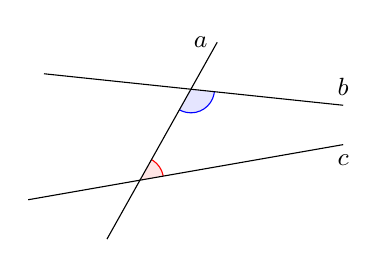
\begin{tikzpicture}[scale=1,font=\small]
\usetikzlibrary{calc}


\begin{scope}
\coordinate (c1) at (0,0);
\coordinate (c2) at (4,0.7);
\coordinate (a1) at (1,-0.5);
\coordinate (a2) at (2.4,2);
\coordinate (b1) at (0.2,1.6);
\coordinate (b2) at (4,1.2);
\coordinate (ab) at (intersection of a1--a2 and b1--b2);
\coordinate (ac) at (intersection of a1--a2 and c1--c2);

\begin{scope}
\clip (b2) -- (ab) -- (ac) -- (c2) -- cycle;
\draw[blue, fill=blue!10] (ab) circle (0.3);
\draw[red, fill=red!10] (ac) circle (0.3);
\end{scope}

\draw (a1) -- (a2) node [left] {$a$};
\draw (b1) -- (b2) node [above] {$b$};
\draw (c1) -- (c2) node [below] {$c$};

\end{scope}


\end{tikzpicture}

 \end{minipage}\hfil
 \begin{minipage}{.45\textwidth}
 Nella figura, la retta $a$ taglia le rette $b$ e $c$, formando sul lato destro due angoli la cui somma è minore di due angoli retti. Prolungando opportunamente le rette $b$ e $c$ risulta che esse si incontrano sul lato destro della figura.
  \end{minipage}
\end{enumerate}

Nell'impostazione assiomatica moderna di Hilbert, gli assiomi hanno la funzione di definire implicitamente gli enti primitivi, cioè di fissare le proprietà alle quali questi enti devono soddisfare. Hilbert aggiunge inoltre altri assiomi che Euclide stesso non aveva esplicitato chiaramente.

\subsubsection*{Assiomi di Hilbert}\label{sect:ass_Hilbert}

L'esposizione che segue è una semplificazione degli assiomi del grande matematico tedesco.\footnote{chi volesse studiare direttamente il testo originale può consultare \url{http://www.gutenberg.org/files/17384/17384-pdf.pdf} [ultima consultazione 20.03.2014].}

Hilbert assume come enti primitivi della geometria piana il \emph{punto} e la \emph{retta}, come relazioni primitive l'appartenenza di un punto ad una retta, il giacere di un punto tra altri due punti, e la congruenza di segmenti.

\paragraph{Assiomi di appartenenza} ``giacere su''
\begin{enumerate}[label=\Roman{*}.]
\item dati due punti distinti, esiste una e una sola retta che contiene entrambi i punti;
\item ogni retta contiene almeno due punti. Esistono almeno tre punti che non giacciono sulla stessa retta (figura~\ref{fig:1.3});
\item dati tre punti non allineati, esiste uno e un solo piano che contiene tutti e tre i punti. Ogni piano contiene almeno un punto (figura~\ref{fig:1.4});
\item se due punti di una retta giacciono su un piano, allora anche tutti gli altri punti della retta giacciono su questo piano (figura~\ref{fig:1.5});
\item se un punto giace su due piani distinti, allora esiste almeno un altro punto giacente su entrambi questi piani;
\item esistono almeno quattro punti che non giacciono sullo stesso piano.
\end{enumerate}

\begin{figure}[b,t,h]
 \begin{minipage}[b]{.32\textwidth}
 \centering
 \begin{tikzpicture}[font=\small]
%Assioma 2
\tkzDefPoint(0,0){O}
\tkzDefShiftPoint[O](20:.7){A}
\tkzDefShiftPoint[O](20:2){B}
\tkzDefShiftPoint[O](20:2.7){M}
\tkzDefShiftPoint[O](50:1.5){C}
\tkzDefShiftPoint[O](30:0){r}
\tkzDrawSegment(O,M)
\tkzDrawPoints(A,B,C)
\tkzLabelPoints[font=\small](A,B,C,r)
% % % % % % % % % % % % % % % % % % % % % % % % % % % % % % % % %
\begin{comment}
%i punti
\tkzDefPoint(0,0){D}
\tkzDefShiftPoint[D](60:2){G}
\tkzDefShiftPoint[G](0:2.5){F}
\tkzDefShiftPoint[D](0:2.5){E}
\tkzDrawPolygon[fill=blue!10](D,G,F,E)
\node at(3.6,1.4){$\pi$};

%le rette
\tkzDefPoint(.5,.5){H}
\tkzDefShiftPoint[H](30:.5){I}
\tkzDefShiftPoint[H](30:1.5){L}
\tkzDefShiftPoint[H](30:2){M}
\tkzDrawSegment(H,M)
\node at(4.3,.5){r};
\node at(4.3,-.5){s};

\tkzDefPoint(3,-1){D}
\tkzDefShiftPoint[D](35:1){E}
\tkzDefShiftPoint[D](35:3){F}
\tkzDefShiftPoint[D](35:4){G}
\tkzDrawSegments[style=dashed](D,E F,G)
\tkzDrawSegment(E,F)
\node at(4,-1-1){rette};
\end{comment}
% % % % % % % % % % % % % % % % % % % % % % % % % % % % % % % % %
\end{tikzpicture}

 \caption{Assioma II}\label{fig:1.3}
 \end{minipage}
 \begin{minipage}[b]{.32\textwidth}
 \centering
 \begin{tikzpicture}[font=\small]
%il piano1
\tkzDefPoint(0,0){D}
\tkzDefShiftPoint[D](60:2){G}
\tkzDefShiftPoint[G](0:2.5){F}
\tkzDefShiftPoint[D](0:2.5){E}
\tkzDrawPolygon[fill=blue!10](D,G,F,E)
\node at(3.6,1.4){$\pi$};
\tkzDefPoint(.9,1){A}
\tkzDefPoint(2.6,1.5){B}
\tkzDefPoint(2.1,.5){C}
\tkzDrawPoints(A,B,C)
\tkzLabelPoints[font=\small](A,B,C)
% % % % % % % % % % % % % % % % % % % % % % % % % % % % % % % % %
\begin{comment}
%i punti
\tkzDefPoint(.2,1){A}
\tkzDefPoint(1.3,1.7){B}
\tkzDefPoint(2.5,.5){C}
\tkzDrawPoints(A,B,C)
\tkzLabelPoints(A,B,C)
\node at(.75,-2){punti};

%le rette
\tkzDefPoint(3,-.5){D}
\tkzDefShiftPoint[D](30:1){E}
\tkzDefShiftPoint[D](30:3){F}
\tkzDefShiftPoint[D](30:4){G}
\tkzDrawSegments[style=dashed](D,E F,G)
\tkzDrawSegment(E,F)
\node at(4.3,.5){r};
\node at(4.3,-.5){s};

\tkzDefPoint(3,-1){D}
\tkzDefShiftPoint[D](35:1){E}
\tkzDefShiftPoint[D](35:3){F}
\tkzDefShiftPoint[D](35:4){G}
\tkzDrawSegments[style=dashed](D,E F,G)
\tkzDrawSegment(E,F)
\node at(4,-1-1){rette};
\end{comment}
% % % % % % % % % % % % % % % % % % % % % % % % % % % % % % % % %
\end{tikzpicture}

 \caption{Assioma III}\label{fig:1.4}
 \end{minipage}
 \begin{minipage}[b]{.32\textwidth}
 \centering
 \begin{tikzpicture}[font=\small]
%il piano1
\tkzDefPoint(0,0){D}
\tkzDefShiftPoint[D](60:2){G}
\tkzDefShiftPoint[G](0:2.5){F}
\tkzDefShiftPoint[D](0:2.5){E}
\tkzDrawPolygon[fill=blue!10](D,G,F,E)
\node at(3.6,1.4){$\pi$};
\tkzDefPoint(.5,.3){H}
\tkzDefShiftPoint[H](25:.7){A}
\tkzDefShiftPoint[H](25:2){B}
\tkzDefShiftPoint[H](25:2.7){M}
\tkzDefShiftPoint[H](35:2.5){r}
\tkzDrawSegment(H,M)
\tkzDrawPoints(A,B)
\tkzLabelPoints[font=\small](A,B,r)
% % % % % % % % % % % % % % % % % % % % % % % % % % % % % % % % %
\begin{comment}
%i punti
\tkzDefPoint(.2,1){A}
\tkzDefPoint(1.3,1.7){B}
\tkzDefPoint(2.5,.5){C}
\tkzDrawPoints(A,B,C)
\tkzLabelPoints(A,B,C)
\node at(.75,-2){punti};

%le rette
\tkzDefPoint(.5,.5){H}
\tkzDefShiftPoint[H](30:.5){I}
\tkzDefShiftPoint[H](30:1.5){L}
\tkzDefShiftPoint[H](30:2){M}
\tkzDrawSegment(H,M)
\node at(4.3,.5){r};
\node at(4.3,-.5){s};

\tkzDefPoint(3,-1){D}
\tkzDefShiftPoint[D](35:1){E}
\tkzDefShiftPoint[D](35:3){F}
\tkzDefShiftPoint[D](35:4){G}
\tkzDrawSegments[style=dashed](D,E F,G)
\tkzDrawSegment(E,F)
\node at(4,-1-1){rette};
\end{comment}
% % % % % % % % % % % % % % % % % % % % % % % % % % % % % % % % %
\end{tikzpicture}

 \caption{Assioma IV}\label{fig:1.5}
 \end{minipage}
\end{figure}

\paragraph{Assiomi di ordinamento} ``stare fra''
\begin{enumerate}[label=\Roman{*}.]
\setcounter{enumi}{6}
\item Se un punto $B$ giace fra i punti $A$ e $C$, allora i punti $A$, $B$ e $C$ sono tre punti distinti sulla stessa retta, e $B$ giace fra $C$ ed $A$ (figura~\ref{fig:1.6});
\item dati due punti $A$ e $C$, esiste almeno un punto $B$, sulla retta $AC$, giacente fra di essi;
\item dati tre punti qualsiasi di una retta, uno e uno solo di essi giace fra gli altri due.
\end{enumerate}
Gli ultimi assiomi ci permettono di dedurre il seguente teorema.
\begin{teorema}
Tra due punti di una retta esiste sempre una quantità illimitata di altri punti.
\end{teorema}
\begin{proof}
Data una retta $r$ e due suoi punti $A$ e $B$, per l'assioma~VIII sappiamo che esiste un terzo punto $C$ sulla retta $r$ che giace tra $A$ e $B$. Ma allora esiste un punto $D$ su $r$ che giace tra $A$ e $C$ e un punto $E$ che giace tra $C$ e $B$. Per lo stesso assioma esisterà un punto tra $A$ e $D$, uno tra $D$ e $C$, uno tra $C$ e $B$ e così via.
\end{proof}
\begin{center}
\begin{tikzpicture}
%Assioma 14
\tkzDefPoint(0,0){L}
\tkzDefShiftPoint[L](0:.3){A}
\tkzDefShiftPoint[L](0:5.7){B}
\tkzDefShiftPoint[L](0:3){C}
\tkzDefShiftPoint[L](0:1.7){D}
\tkzDefShiftPoint[L](0:4.3){E}
\tkzDefShiftPoint[L](0:6){M}
\tkzDefShiftPoint[L](0:6){r}
\tkzDrawSegment(L,M)
\tkzDrawPoints(A,B,C,D,E)
\tkzLabelPoints[font=\small, above](A,B,C,D,E)
\tkzLabelPoint[font=\small](r){r}
\end{tikzpicture}

\end{center}
\begin{definizione}
Si chiama \emph{segmento} $AB$ l'insieme dei punti $A$ e $B$ e di tutti quelli che stanno sulla retta tra $A$ e $B$.
\end{definizione}
Gli assiomi di ordinamento ci permettono di dare anche la seguente

\begin{definizione}
Presi quattro punti $A$, $B$, $C$, $O$ su una retta, in modo che $B$ stia tra $A$ e $O$ e $O$ stia tra $A$ e $C$ possiamo dire che $A$ e $B$ \emph{stanno dalla medesima parte} rispetto a $O$, mentre $A$ e $C$ non stanno dalla medesima parte rispetto a $O$.
\end{definizione}
\begin{center}
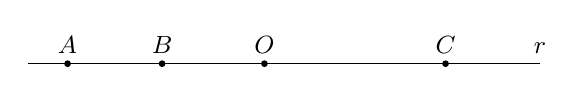
\begin{tikzpicture}[scale=1,font=\small]
\usetikzlibrary{calc}

\begin{scope}
\coordinate (l) at (0,0);
\path (l) -- +(0:.5) coordinate (a);
\path (l) -- +(0:1.7) coordinate (b);
\path (l) -- +(0:5.3) coordinate (c);
\path (l) -- +(0:3) coordinate (o);
\path (l) -- +(0:4.3) coordinate (e);
\path (l) -- +(0:6.5) coordinate (m);

\draw (l) -- (m) node [above] {$r$};

\draw[fill] (a) circle (1pt) node [above] {$A$};
\draw[fill] (b) circle (1pt) node [above] {$B$};
\draw[fill] (c) circle (1pt) node [above] {$C$};
\draw[fill] (o) circle (1pt) node [above] {$O$};

\end{scope}

\end{tikzpicture}

\end{center}

\osservazione Trascuriamo in questa trattazione elementare l'assioma di Pasch\footnote{Moritz Pasch è stato un matematico tedesco (1843 - 1930).} (X) e l'assioma delle parallele (XI).

\paragraph{Assiomi di congruenza} ``essere congruente a''
\begin{enumerate}[label=\Roman{*}.]
\setcounter{enumi}{11}
\item \emph{Assioma del trasporto di un segmento}. Se $A$, $B$ sono due punti di una retta $r$ e $A'$ è un punto sulla stessa retta (o fissato su un'altra retta $r'$), si può sempre trovare un punto $B'$ sulla retta $r$ (o su $r'$), da una data parte rispetto ad $A'$, tale che il segmento $AB$ sia congruente al segmento $A'B'$;
\item la relazione di congruenza tra segmenti è transitiva, cioè se $A'B'$ è congruente ad $AB$ e $A''B''$ è congruente ad $AB$ allora $A'B'$ è congruente ad $A''B''$ (figura~\ref{fig:1.7});
\item siano $AB$ e $BC$ segmenti su una retta $r$ privi di punti comuni a parte $B$, e siano $A'B'$ e $B'C'$ segmenti su una retta $r'$ privi di punti comuni a parte $B'$. Se $AB\equiv A'B'$ e $BC\equiv B'C'$, allora  $AC\equiv A'C'$ (figura~\ref{fig:1.8}).
\end{enumerate}

\begin{figure}[b,t,h]
 \begin{minipage}[b]{.28\textwidth}
 \centering
 \begin{tikzpicture}
%Assioma 7
\tkzDefPoint(0,0){O}
\tkzDefShiftPoint[O](0:.5){A}
\tkzDefShiftPoint[O](0:1.2){B}
\tkzDefShiftPoint[O](0:1.9){C}
\tkzDefShiftPoint[O](0:2.5){M}
\tkzDefShiftPoint[O](0:2.5){r}
\tkzDrawSegment(O,M)
\tkzDrawPoints(A,B,C)
\tkzLabelPoints[font=\small, above](A,B,C)
\tkzLabelPoint[font=\small](r){$r$}
\end{tikzpicture}

 \caption{Assioma VII}\label{fig:1.6}
 \end{minipage}
 \begin{minipage}[b]{.34\textwidth}
 \centering
 \begin{tikzpicture}
%Assioma 12
\tkzDefPoint(0,0){L}
\tkzDefShiftPoint[L](0:.6){A}
\tkzDefShiftPoint[L](0:1.1){B}
\tkzDefShiftPoint[L](0:2){A'}
\tkzDefShiftPoint[L](0:2.5){B'}
\tkzDefShiftPoint[L](0:3){M}
\tkzDefShiftPoint[L](0:3){r}
\tkzDrawSegment(L,M)
\tkzDrawPoints(A,B,A',B')
\tkzLabelPoints[font=\small, above](A,B,A',B')
\tkzLabelPoint[font=\small](r){r}
\end{tikzpicture}

 \caption{Assioma XII}\label{fig:1.7}
 \end{minipage}
 \begin{minipage}[b]{.34\textwidth}
 \centering
 \begin{tikzpicture}
%Assioma 14
\tkzDefPoint(0,0){L}
\tkzDefShiftPoint[L](0:.6){A}
\tkzDefShiftPoint[L](0:1.5){B}
\tkzDefShiftPoint[L](0:2){C}
\tkzDefShiftPoint[L](0:3){M}
\tkzDefShiftPoint[L](0:3){r}
\tkzDrawSegment(L,M)
\tkzDrawPoints(A,B,C)
\tkzLabelPoints[font=\small, above](A,B,C)
\tkzLabelPoint[font=\small](r){r}

\tkzDefPoint(0,-.7){L}
\tkzDefShiftPoint[L](0:.6){A'}
\tkzDefShiftPoint[L](0:1.5){B'}
\tkzDefShiftPoint[L](0:2){C'}
\tkzDefShiftPoint[L](0:3){M}
\tkzDefShiftPoint[L](0:3){r'}
\tkzDrawSegment(L,M)
\tkzDrawPoints(A',B',C')
\tkzLabelPoints[font=\small, above](A',B',C')
\tkzLabelPoint[font=\small](r'){r'}
\end{tikzpicture}

 \caption{Assioma XIV}\label{fig:1.8}
 \end{minipage}
\end{figure}

Prima di proseguire con gli altri assiomi premettiamo le seguenti definizioni.
\begin{definizione}
Chiamiamo \emph{semiretta} la parte di retta costituita da un punto di essa, detto origine della semiretta, e da tutti i punti che stanno dalla stessa parte rispetto all'origine.
\end{definizione}

\begin{center}
 \begin{tikzpicture}
%Semiretta
\tkzDefPoint(0,0){O}
\tkzDefShiftPoint[O](0:5){C}
\tkzDefShiftPoint[O](0:6){M}
\tkzDrawSegment(O,C)
\tkzDrawSegment[style=dashed](C,M)
\tkzDrawPoint(O)
\tkzLabelPoint[font=\small, above](O){$O$}
\end{tikzpicture}

\end{center}

\begin{definizione}
Si dice \emph{angolo} ciascuna delle due parti in cui un piano è diviso da due semirette aventi l'origine in comune; le semirette si dicono \emph{lati} dell'angolo; l'origine comune alle due semirette si dice \emph{vertice} dell'angolo (figura~\ref{fig:1.9}).
\end{definizione}
\begin{figure*}[b,t,h]
\centering  \begin{tikzpicture}
%angolo1
\tkzDefPoint(0,0){H}
\tkzDefPoint(0,3){I}
\tkzDefShiftPoint[H](0:6){M}
\tkzDefShiftPoint[I](0:6){L}
\tkzDefPoint(2,1.5){V}
\tkzDefMidPoint(V,L)	\tkzGetPoint{M1}
\tkzDefMidPoint(V,M)	\tkzGetPoint{M2}
\tkzDrawSegments(V,L V,M)
\tkzFillPolygon[yellow!30](L,V,M,H,I)
\tkzFillPolygon[blue!30,opacity=.25](L,V,M)
%\tkzDrawSegment[style=dashed](C,M)
\tkzDrawPoint(V)
\tkzLabelPoint[above right](1,.3){Angolo}
\tkzLabelPoint[right](3.5,1.5){Angolo}
\tkzLabelPoint[font=\small, left](V){vertice}
\tkzLabelPoint[font=\small, above](V){V}
\tkzLabelPoint[font=\small, above](M1){lato}
\tkzLabelPoint[font=\small, below](M2){lato}
\tkzLabelPoint[font=\small, below left](L){r}
\tkzLabelPoint[font=\small, above left](M){s}
\end{tikzpicture}

\caption{Le semirette $r$ e $s$, aventi l'origine $V$ comune, individuano due regioni del piano ognuna delle quali è detta angolo.}\label{fig:1.9}
\end{figure*}

L'angolo individuato da tre punti $A$, $B$, $C$ è l'angolo formato dalla semiretta con origine $B$ e passante per $A$ e dalla semiretta con origine $B$ e passante per $C$. Questo angolo si indica con il simbolo $A\widehat{B}C$. Nei disegni si usa indicare l'angolo con un archetto che indica la parte di piano considerata.

\begin{enumerate}[label=\Roman{*}.]
\setcounter{enumi}{14}
\item Dati un angolo $A\widehat{B}C$ ed una semiretta $B'C'$, esistono e sono uniche due semirette $B'D$ e $B'E$, tali che l'angolo $D\widehat{B'}C'$ è congruente all'angolo $A\widehat{B}C$ e l'angolo $E\widehat{B'}C'$ è congruente all'angolo $A\widehat{B}C$ (figura~\ref{fig:1.10});
\begin{figure}[b,t,h]
 \centering \begin{tikzpicture}
%assioma 15
\tkzDefPoint(0,0){B}
\tkzDefShiftPoint[B](0:2.5){A}
\tkzDefShiftPoint[B](0:3){I}
\tkzDefShiftPoint[B](30:2.5){C}
\tkzDefShiftPoint[B](30:3){H}
\tkzDrawPoints(A,B,C)
\tkzDrawSegments(B,H B,I)
\tkzLabelPoints[font=\small](B,C,A)
\tkzMarkAngle[fill=orange,opacity=.3,size=1cm](A,B,C)

\tkzDefShiftPoint[B](0:5){B'}
\tkzDefShiftPoint[B'](0:2.5){C'}
\tkzDefShiftPoint[B'](0:3){M}
\tkzDefShiftPoint[B'](30:2.5){E}
\tkzDefShiftPoint[B'](30:3){L}
\tkzDefShiftPoint[B'](-30:2.5){D}
\tkzDefShiftPoint[B'](-30:3){N}
\tkzDrawPoints(B',E,C',D)
\tkzDrawSegments(B',L B',M B',N)
\tkzLabelPoints[font=\small](E,C')
\tkzLabelPoints[font=\small,below](B',D)
\tkzMarkAngle[fill=orange,opacity=.3,size=1cm](D,B',C')
\tkzMarkAngle[fill=orange,opacity=.3,size=.9cm](C',B',E)

% % % % % %
\begin{comment}
\tkzDefShiftPoint[I](0:4){L}
\tkzDefPoint(1.5,1){V}
\tkzDefMidPoint(V,L)	\tkzGetPoint{M1}
\tkzDefMidPoint(V,M)	\tkzGetPoint{M2}
\tkzDrawSegments(V,L V,M)
\tkzFillPolygon[red!30,opacity=.25](L,V,M,H,I)
\tkzFillPolygon[blue!30,opacity=.25](L,V,M)
%\tkzDrawSegment[style=dashed](C,M)
\tkzDrawPoint(V)
\tkzLabelPoint[above right](.5,.1){Angolo}
\tkzLabelPoint[right](2.5,1){Angolo}
\tkzLabelPoint[font=\small, left](V){vertice}
\tkzLabelPoint[font=\small, above](V){V}
\tkzLabelPoint[font=\small, above](M1){lato}
\tkzLabelPoint[font=\small, below](M2){lato}
\tkzLabelPoint[font=\small, below left](L){r}
\tkzLabelPoint[font=\small, above left](M){s}
% % % % % % %
\end{comment}
\end{tikzpicture}

 \caption{Assioma XV}\label{fig:1.10}
\end{figure}
\item La relazione di congruenza tra angoli è transitiva, cioè se  $A'\widehat{B'}C'$ e  $A''\widehat{B''}C''$ sono congruenti ad $A\widehat{B}C$, allora  $A'\widehat{B'}C' \equiv A''\widehat{B''}C''$.
\end{enumerate}

\paragraph{Assioma di continuità}

\begin{enumerate}[label=\Roman{*}.]
\setcounter{enumi}{16}
\item \emph{Assioma di Archimede}. Sulla retta che unisce due punti qualsiasi $A$ e $B$ si prende un punto $A_1$, quindi si prendono i punti $A_2$, $A_3$, $A_4$, \ldots in modo che $A_1$ sia tra $A$ e $A_2$, $A_2$ tra $A_1$ e $A_3$, $A_3$ tra $A_2$ e $A_4$, ecc. e che  $AA_1\equiv A_1A_2\equiv A_2A_3\equiv A_3A_4\equiv\ldots$ allora tra tutti questi punti esiste sempre un punto $A_n$ tale che $B$ sta tra $A$ e $A_n$ (figura~\ref{fig:1.11}).
\begin{figure}[b,t,h]
 \centering \begin{tikzpicture}
%assioma 15
\tkzDefPoint(0,0){O}
\tkzDefShiftPoint[O](0:8){O'}
\tkzDefShiftPoint[O](0:5.1){B}
\tkzDefShiftPoint[O](0:1){A}
\tkzDefShiftPoint[O](0:1.9){A1}
\tkzDefShiftPoint[O](0:2.8){A2}
\tkzDefShiftPoint[O](0:3.7){A3}
\tkzDefShiftPoint[O](0:4.6){A4}
\tkzDefShiftPoint[O](0:5.5){A5}
\tkzDefShiftPoint[O](0:6.4){A6}
\tkzDefShiftPoint[O](0:7.4){A7}
\tkzDrawPoints(A1,A2,A3,A4,A5,A6,A7)
\tkzDrawPoints[fill=red,size=8](B,A)
\tkzDrawSegment(O,O')
\tkzLabelPoint[above](A){$A$}
\tkzLabelPoint[above](B){$B$}
\tkzLabelPoint[font=\small,above](A1){$A_1$}
\tkzLabelPoint[font=\small,above](A2){$A_2$}
\tkzLabelPoint[font=\small,above](A3){$A_3$}
\tkzLabelPoint[font=\small,above](A4){$A_4$}
\tkzLabelPoint[font=\small,above](A5){$A_5$}
\tkzLabelPoint[font=\small,above](A6){$A_6$}
\tkzLabelPoint[font=\small,above](A7){$A_7$}
\tkzLabelPoint[font=\small](7.8,0){$r$}
\end{tikzpicture}

 \caption{Assioma XVII di Archimede}\label{fig:1.11}
\end{figure}
\end{enumerate}

\paragraph{Assioma di completezza}

\begin{enumerate}[label=\Roman{*}.]
\setcounter{enumi}{17}
\item Ad un sistema di punti, linee rette e piani è impossibile aggiungere altri elementi in modo tale che il sistema, così generalizzato, formi una nuova geometria obbediente a tutti i cinque gruppi di assiomi. In altre parole, gli elementi della geometria formano un sistema che non è suscettibile di estensione, nel caso in cui si considerino validi i cinque gruppi di assiomi.
\end{enumerate}

\section{Prime definizioni}

Nel paragrafo precedente abbiamo già introdotto alcune definizioni di base, necessarie per enunciare tutti i postulati della geometria secondo l'assiomatizzazione di Hilbert. In questo paragrafo costruiamo le prime definizioni. Per comodità del lettore riportiamo anche quelle già date.

Partiamo dalla nozione generica di figura.
\begin{definizione}
Si chiama \emph{figura} un qualsiasi insieme, non vuoto, di punti.
\end{definizione}
Questa definizione fa riferimento soltanto all'ente primitivo geometrico di punto.

Lo spazio non è considerato un ente primitivo, in quanto può essere ottenuto dalla seguente definizione.
\begin{definizione}
Si chiama \emph{spazio} l'insieme di tutti i punti.
\end{definizione}
Risulta pertanto che una figura è un qualsiasi sottoinsieme dello spazio.

In base agli assiomi di ordinamento un qualunque punto $P$ su una retta divide la retta in due parti, una è costituita dai punti che ``seguono'' $P$, l'altra è costituita dai punti che ``precedono'' $P$.
\begin{definizione}
Si chiama \emph{semiretta} la parte di retta costituita da un punto di essa, detto origine della semiretta, e da tutti i punti che stanno dalla stessa parte rispetto all'origine.
\end{definizione}
Solitamente, la semiretta si indica con una lettera latina minuscola.

Prendendo due qualsiasi rette dello spazio esse si possono trovare in diverse posizioni reciproche, cioè una rispetto all'altra.
\begin{definizione}
Due rette si dicono \emph{complanari} se appartengono a uno stesso piano; se non appartengono a uno stesso piano si dicono \emph{sghembe}.

Due rette complanari si dicono \emph{incidenti} se hanno uno, e uno solo, punto in comune.

Due rette complanari che non hanno nessun punto in comune si dicono \emph{parallele}.

Se due rette hanno almeno due punti in comune sono \emph{coincidenti} (figura~\ref{fig:1.12}).
\end{definizione}
\begin{figure}[b,t,h]
 \centering 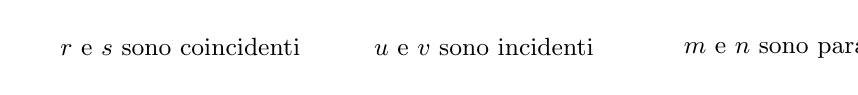
\begin{tikzpicture}[font=\small]
%rette coincidenti
\tkzDefPoint(0,0){A}
\tkzDefShiftPoint[A](20:3){B}
\tkzDefPoint(0,-.05){C}
\tkzDefShiftPoint[C](20:3){D}
\tkzLabelPoint[font=\small,above](B){$ r $}
\tkzLabelPoint[font=\small,below](D){$ s $}
\tkzDrawSegments(A,B C,D)
\node at(1.5,-1){$ r $ e $ s $ sono coincidenti};

%rette incidenti
\tkzDefPoint(3.5,0){A}
\tkzDefShiftPoint[A](20:3){B}
\tkzDefPoint(4,-.3){C}
\tkzDefShiftPoint[C](40:2.5){D}
\tkzLabelPoint[font=\small,below](B){$ v $}
\tkzLabelPoint[font=\small,above](D){$ u $}
\tkzDrawSegments(A,B C,D)
\node at(5,-1){$ u $ e $ v $ sono incidenti};

%rette parallele
\tkzDefPoint(7,0){A}
\tkzDefShiftPoint[A](30:3){B}
\tkzDefPoint(7.5,-.3){C}
\tkzDefShiftPoint[C](30:3){D}
\tkzLabelPoint[font=\small,above](B){$ m $}
\tkzLabelPoint[font=\small,below](D){$ n $}
\tkzDrawSegments(A,B C,D)
\node at(8.5,-1){$ m $ e $ n $ sono parallele};
\end{tikzpicture}

 \caption{Relazioni tra rette complanari}\label{fig:1.12}
\end{figure}
Per indicare che le rette $r$ e $s$ sono parallele si usa il simbolo $r \parallel s$.

\osservazione Due rette non parallele possono appartenere a piani diversi, in questo caso non avranno punti in comune, sono cioè sghembe. Viceversa se due rette hanno un punto in comune allora sono sicuramente complanari. Inoltre, se hanno più di un punto in comune le rette coincidono, in questo caso ci sono infiniti piani che le contengono. 

\begin{definizione}
L'insieme di tutte le rette di un piano che passano per uno stesso punto è detto \emph{fascio proprio di rette}, il punto in comune a tutte le rette si dice centro del fascio (figura~\ref{fig:1.16}).
\end{definizione}

Prendendo due punti su una retta, $A$ e $B$, la retta resta divisa in tre parti: la semiretta di origine $A$ che non contiene $B$, la parte costituita dai punti compresi tra $A$ e $B$ e la semiretta di origine $B$ che non contiene $A$.

\begin{definizione}
Si chiama \emph{segmento} $AB$ l'insieme dei punti $A$ e $B$ e di tutti quelli che stanno tra $A$ e $B$.
I punti $A$ e $B$ si dicono \emph{estremi} del segmento.
\end{definizione}
Un segmento viene indicato con le due lettere maiuscole dei suoi estremi.
\begin{figure}[bth]
 \centering \begin{tikzpicture}[font=\small]
%definizione di segmento
\tkzDefPoint(0,0){r}
\tkzDefShiftPoint[r](0:9){s}
\tkzDefShiftPoint[r](0:3){A}
\tkzDefShiftPoint[r](0:6){B}
\tkzDefPoint(1.5,.5){e1}
\tkzDefPoint(7.5,.5){e2}
\tkzDefPoint(4.5,0){p}
\tkzDefPoint(1.5,-.5){s1}
\tkzDefPoint(7.5,-.5){s2}
\tkzDrawSegments[style=dashed](r,A B,s)
\tkzDrawSegment[very thick](A,B)
\tkzDrawPoints[fill=red](A,B)
\tkzLabelPoints[font=\small,above](r,s)
\tkzLabelPoints[font=\small,above](A,B)
\tkzLabelPoint[font=\small,above](p){punti interni}
\tkzLabelPoint[font=\small,below](4.5,-.5){segmento $AB$}
\tkzLabelPoint[font=\small,below](s1){semiretta di origine $A$}
\tkzLabelPoint[font=\small,below](s2){semiretta di origine $B$}
\tkzLabelPoint[font=\small,above](e1){estremo}
\tkzLabelPoint[font=\small,above](e2){estremo}
\tkzDrawSegments[thick,dotted,->,-latex](e1,A e2,B)
\tkzDrawSegment[thick,dotted,->,-latex]({4.5,-.5},{4.5,0})
%\draw[thick,dotted,->,-latex](0.5,-0.5).. controls (2,-.2)..(1,0);
%\draw[thick,dotted,->,-latex](8.5,-0.5).. controls (7,-.2)..(8,0);
\tkzDefPoint(1.5,0){rm}
\tkzDrawSegments[thick,dotted,->,-latex](s1,rm)
\tkzDefPoint(7.5,0){sm}
\tkzDrawSegments[thick,dotted,->,-latex](s2,sm)
\end{tikzpicture}

 \caption{I punti $A$ e $B$ formano le due semirette $r$ e $s$, e il segmento $AB$}\label{fig:1.12}
\end{figure}

Due segmenti nel piano possono trovarsi in diverse posizioni reciproche. Alcune di esse hanno un interesse per la geometria.
\begin{definizione}
Due segmenti si dicono \emph{consecutivi} se hanno in comune soltanto un estremo (figura~\ref{fig:1.14}).
\end{definizione}
\begin{figure}[bth]
 \centering % Copyright (c) 2015 Daniele Masini - d.masini.it@gmail.com

\begin{tikzpicture}[font=\small]
%segmenti consecutivi
\tkzDefPoint(0,0){B}
\tkzDefShiftPoint[B](120:2){A}
\tkzDefShiftPoint[B](0:2.5){C}
\tkzDrawPoints(A,B,C)
\tkzLabelPoints[font=\small](B,C)
\tkzLabelPoint[font=\small,right](A){A}
\tkzDrawSegments(A,B B,C)
\node at(1.25,-.7){segmenti consecutivi};

%non consecutivi
\tkzDefPoint(4,0){E}
\tkzDefShiftPoint[E](120:.7){F}
\tkzDefShiftPoint[E](120:2){D}
\tkzDefShiftPoint[F](10:2.5){G}
\tkzDrawPoints(E,F,D,G)
\tkzLabelPoints[font=\small,left](E,F,D)
\tkzLabelPoint[font=\small,above](G){G}
\tkzDrawSegments(E,D F,G)
\node at(6.5,-.7){Segmenti non consecutivi};

\tkzDefPoint(7,0){H}
\tkzDefShiftPoint[H](100:2){I}
\tkzDefShiftPoint[H](60:1.5){L}
\tkzDefShiftPoint[H](10:3){M}
\tkzDrawPoints(H,I,L,M)
\tkzLabelPoints[font=\small,right](H,I)
\tkzLabelPoints[font=\small,above](L,M)
\tkzDrawSegments(H,I L,M)
\end{tikzpicture}

 \caption{I segmenti $AB$ e $BC$ sono consecutivi perché hanno in comune solo il punto~$B$ che è un estremo di entrambi; $DE$ e $FG$ non sono consecutivi perché hanno in comune solo il punto $F$ ma esso non è estremo del segmento $DE$; $HI$ e $LM$ non sono consecutivi perché non hanno nessun punto in comune.}\label{fig:1.14}
\end{figure}

\begin{definizione}
Due segmenti si dicono \emph{adiacenti} se sono consecutivi ed appartengono alla stessa retta (figura~\ref{fig:1.15}).
\end{definizione}
\begin{figure}[tbh]
 \centering % Copyright (c) 2015 Daniele Masini - d.masini.it@gmail.com

\begin{tikzpicture}[font=\small]
%segmenti adiacenti
\tkzDefPoint(0,0){A}
\tkzDefShiftPoint[A](60:1.5){B}
\tkzDefShiftPoint[A](60:2.5){C}
\tkzDrawPoints(A,B,C)
\tkzLabelPoints[font=\small,right](A,B,C)
\tkzDrawSegment(A,C)
\node at(.3,-.5){segmenti adiacenti};

%non consecutivi
\tkzDefPoint(4,0){D}
\tkzDefShiftPoint[D](60:.7){E}
\tkzDefShiftPoint[D](60:1.7){F}
\tkzDefShiftPoint[D](60:2.5){G}
\tkzDrawPoints(E,F,D,G)
\tkzLabelPoints[font=\small,right](D,E,F,G)
\tkzDrawSegments(E,D F,G)
\tkzDrawSegment[dashed](E,F)
\node at(5.5,-.5){Segmenti non adiacenti};

\tkzDefPoint(7,0){H}
\tkzDefShiftPoint[H](60:1){L}
\tkzDefShiftPoint[H](60:1.5){I}
\tkzDefShiftPoint[H](60:2.5){M}
\tkzDrawPoints(H,I,L,M)
\tkzLabelPoints[font=\small,right](H,I,L,M)
\tkzDrawSegment(H,M)
\end{tikzpicture}

 \caption{I segmenti $AB$ e $BC$ sono adiacenti perché hanno in comune solo l'estremo $B$ e giacciono sulla stessa retta; i segmenti $DE$ e $FG$, pur giacendo sulla stessa retta, non sono adiacenti poiché non hanno alcun punto in comune; i segmenti $HI$ e $LM$ giacciono sulla stessa retta ma non sono adiacenti poiché hanno più di un punto in comune.}\label{fig:1.15}
\end{figure}

\subsection{Semipiani e angoli}

\begin{definizione}
Si dice \emph{semipiano} di origine la retta $r$ la figura formata dalla retta $r$ e da una delle due parti in cui essa divide il piano (figura~\ref{fig:1.17}).
\end{definizione}
\begin{figure}[b,t,h]
 \begin{minipage}[b]{.40\textwidth}
 \centering\begin{tikzpicture}[font=/small]
\tkzDefPoint(0,0){O}
%\tkzDefPoint(2,0){A}
\foreach \ang in {30,60,...,360}{%
\tkzDefPoint(\ang:1.3){M}
\tkzDrawSegment(M,O)
}
\end{tikzpicture}

 \caption{Fascio proprio di rette}\label{fig:1.16}
 \end{minipage}\hfil
 \begin{minipage}[b]{.40\textwidth}
 \centering% (c) 2014 Daniele Masini - d.masini.it@gmail.com
\begin{tikzpicture}[font=\small]
%semipiani
\tkzDefPoint(0,0){D}
\tkzDefShiftPoint[D](50:2){G}
\tkzDefShiftPoint[G](0:2.5){F}
\tkzDefShiftPoint[D](0:2.5){E}
\tkzDefShiftPoint[D](50:.7){L}
\tkzDefMidPoint(F,E) \tkzGetPoint{M}
\tkzLabelPoint[right](M){$r$}
\tkzLabelPoint[right](F){$\pi$}
\tkzDrawPolygon[thin,blue,fill=blue!10](L,G,F,M)
\tkzDrawPolygon[thin,blue,fill=yellow!30](D,L,M,E)
\tkzDrawSegment[thick](L,M)
\node at(1.6,.3){semipiano};
\node at(2.1,1.2){semipiano};
\end{tikzpicture}

  \caption{Semipiani opposti}\label{fig:1.17}
  \end{minipage}
\end{figure}
In un piano ${\pi}$, una qualsiasi retta $r \subset \pi$ dà origine a due semipiani distinti, che si dicono semipiani \emph{opposti}.

\begin{definizione}
Una figura si dice \emph{convessa} se, considerati due suoi qualsiasi punti, il segmento che li unisce è contenuto nella figura. Si dice \emph{concava} se esistono almeno due punti per i quali il segmento che li unisce non è interamente contenuto nella figura (figura~\ref{fig:1.18}).
\end{definizione}
\begin{figure}[b,t,h]
 \centering \begin{tikzpicture}[font=\small]
%convesso
\tkzDefPoints{0/1/A,
1.4/.8/B,
3.5/2/C,
1.6/3.2/D,
.6/2/E}
\tkzDefShiftPoint[A](30:.5){A1}
\tkzDefShiftPoint[A1](40:2.1){D1}
\tkzDefShiftPoint[A1](5:.5){A2}
\tkzDefShiftPoint[A1](10:2.1){D2}
\tkzLabelPoint[below,font=\small](1.8,0.85){$F$}
%concavo
\tkzDefPoints{5/2.6/H,
5.8/3/I,
7/2/L,
8.2/2.8/M,
8.5/1.3/N,
8/.3/O,
7/.2/P,
6/.3/Q,
5/.8/R,
5.2/1.7/S}
\tkzDefShiftPoint[H](-3:.7){H1}
\tkzDefShiftPoint[M](-110:.6){M1}
\tkzDefShiftPoint[H](-60:.7){H2}
\tkzDefShiftPoint[L](-40:1){L1}
\tkzDefShiftPoint[R](-10:.5){Q1}
\tkzDefShiftPoint[Q1](10:2.5){Q2}
\tkzLabelPoint[below,font=\small](6.7,0.2){$G$}

\tkzDrawPolygon[fill=blue!10,rounded corners](A,B,C,D,E)
\tkzDrawPolygon[fill=yellow!30,rounded corners](H,I,L,M,N,O,P,Q,R,S)
\tkzDrawSegments(A1,D1 A2,D2 H1,M1 H2,L1 Q1,Q2)
\tkzDrawPoints(A1,D1,A2,D2,H1,M1,H2,L1,Q1,Q2)
\tkzLabelPoint[below,font=\small](H1){$P$}
\tkzLabelPoint[below,font=\small](M1){$Q$}

\end{tikzpicture}


 \caption{La figura $ F $ è convessa, per qualsiasi coppia di punti interni a $ F $ il segmento che li unisce è interamente nella figura; la figura $ G $ è concava perché unendo i punti $ P $ e $ Q $ si ha un segmento che cade in parte esternamente alla figura.}\label{fig:1.18}
\end{figure}

Ricordiamo la definizione di angolo già data: si dice \emph{angolo} ciascuna delle due parti in cui un piano è diviso da due semirette aventi l'origine in comune; le semirette si dicono \emph{lati} dell'angolo; l'origine comune alle due semirette si dice \emph{vertice} dell'angolo (figura~\ref{fig:1.9}).

\begin{definizione}
Un angolo si dice \emph{piatto} se i suoi lati sono uno il prolungamento dell'altro.
Un angolo si dice \emph{nullo} se è costituito solo da due semirette sovrapposte.
\`E detto \emph{angolo giro} l'angolo che ha per lati due semirette sovrapposte e che contiene tutti i punti del piano (figura~\ref{fig:1.19}).
\end{definizione}
\begin{figure}[bth]
 \centering \begin{tikzpicture}
%angolo piatto
\tkzDefPoint(0,0){a}
\tkzDefShiftPoint[a](0:3){b}
\tkzDefShiftPoint[a](0:1.5){V}
\tkzDefShiftPoint[B](30:2.5){C}
\tkzDefShiftPoint[B](30:3){H}
\tkzDrawPoints(a,V,b)
\tkzDrawSegment(a,b)
\tkzLabelPoints[font=\small,below](a,V,b)
\tkzMarkAngle[fill=orange,opacity=.3,size=.8cm](a,V,b)
\tkzMarkAngle[fill=blue!30,opacity=.3,size=.7cm](b,V,a)
\tkzLabelPoint[font=\small,above](1.5,.7){angolo piatto}
\tkzLabelPoint[font=\small,below](1.5,-.8){angolo piatto}
%angolo giro/nullo
\tkzDefShiftPoint[a](0:5){O}
\tkzDefPoint(5,.05){O1}
\tkzDefShiftPoint[O](0:2.5){c}
\tkzDefShiftPoint[O1](0:2.5){c1}
\tkzDefShiftPoint[O](-1:1.5){c2}
\tkzDrawPoint(O)
\tkzDrawSegments(O,c O1,c1)
\tkzLabelPoint[font=\small,above](5,.7){angolo giro}
\tkzLabelPoint[font=\small,below](6.7,0){angolo nullo}
\tkzMarkAngle[fill=orange,opacity=.3,size=.7cm](c,O,c2)
\end{tikzpicture}

 \caption{L'angolo  $\widehat{ab}$ a sinistra è piatto (sia quello sopra che quello sotto), gli angoli a destra, individuati dalle semirette coindicenti con origine in $O$, sono rispettivamente un angolo giro e un angolo nullo.}\label{fig:1.19}
\end{figure}

\begin{definizione}
Un angolo, i cui lati non appartengono alla stessa retta, si dice \emph{concavo} se contiene i prolungamenti dei lati, se non li contiene si dice \emph{convesso}.
\end{definizione}

\begin{figure*}[htb]
\centering  % (c) 2014 Daniele Masini - d.masini.it@gmail.com
\begin{tikzpicture}
%angolo1
\tkzDefPoint(0,0){H}
\tkzDefPoint(0,3){I}
\tkzDefShiftPoint[H](0:6){M}
\tkzDefShiftPoint[I](0:6){L}
\tkzDefPoint(2,1.5){V}
\tkzDefMidPoint(V,L)	\tkzGetPoint{M1}
\tkzDefMidPoint(V,M)	\tkzGetPoint{M2}
\tkzDrawSegments(V,L V,M)
\tkzFillPolygon[yellow!30](L,V,M,H,I)
\tkzFillPolygon[blue!30,opacity=.25](L,V,M)
%\tkzDrawSegment[style=dashed](C,M)
\tkzDrawPoint(V)

\begin{scope}
\clip(0,0) rectangle (3,3);
\tkzDefShiftPoint[H](0:-3){M1}
\tkzDefShiftPoint[I](0:-3){L1}
\tkzDrawSegments[dotted](V,M1 V,L1)
\end{scope}

\tkzLabelPoint[above right](0.7,.3){angolo concavo}
\tkzLabelPoint[right](3,1.5){angolo convesso}

\end{tikzpicture}

\caption{L'angolo concavo è quello in giallo in quanto contiene i prolungamenti dei lati (punteggiati)}\label{fig:1.20}
\end{figure*}

Quando si disegna un angolo è utile, oltre a disegnare le semirette e l'origine, indicare con un archetto quale dei due angoli si intende considerare.

\begin{figure}[htb]
 \centering % Copyright (c) 2015 Daniele Masini - d.masini.it@gmail.com

\begin{tikzpicture}
%assioma 15
\tkzDefPoint(0,0){O}
\tkzDefShiftPoint[O](0:2.5){B}
\tkzDefShiftPoint[O](0:3){I}
\tkzDefShiftPoint[O](30:2.5){A}
\tkzDefShiftPoint[O](30:3){H}
\tkzDrawPoints(A,O,B)
\tkzDrawSegments(O,H O,I)
\tkzLabelPoints[font=\small, left](O)
\tkzLabelPoints[font=\small, above](A)
\tkzLabelPoints[font=\small, below](B)
\tkzMarkAngle[fill=orange,opacity=.3,size=1cm](B,O,A)
\tkzLabelPoint[font=\small,right](19:0.95){$\alpha$}
\tkzLabelPoint[font=\small,above](30:3){$a$}
\tkzLabelPoint[font=\small,below](0:3){$b$}
\end{tikzpicture}

\caption{Per indicare che l'angolo da considerare è quello convesso e non quello concavo si è usato un archetto in prossimità del vertice $O$}\label{fig:1.21}
\end{figure}

Per indicare gli angoli si usano diverse convenzioni:
\begin{itemize}
\item  $\widehat{ab}$ se si conoscono i nomi delle semirette che ne costituiscono i lati;
\item  $A\widehat{O}B$ se si conoscono i nomi del vertice e di due punti sui lati;
\item  $\alpha$, $\beta$, $\gamma$, \ldots{} una lettera greca per indicare direttamente l'angolo.
\end{itemize}
I primi due modi di indicare l'angolo non individuano con chiarezza di quale dei due angoli si tratta. Solitamente si intende l'angolo convesso, quando si vuole indicare l'angolo concavo bisogna dirlo esplicitamente.

Anche per gli angoli si danno le definizioni di angoli consecutivi e angoli adiacenti, in parte simili a quelle date per i segmenti.

\begin{definizione}
Due angoli si dicono angoli \emph{consecutivi} se hanno il vertice e un lato comune e giacciono da parte opposta rispetto al lato comune.
\end{definizione}

\begin{figure}[htb]
 \centering % Copyright (c) 2015 Daniele Masini - d.masini.it@gmail.com

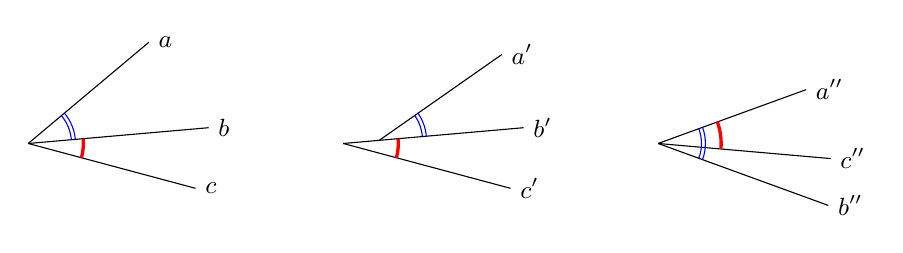
\begin{tikzpicture}
\pgfmathsetmacro{\myscale}{1};

\begin{scope}[scale={\myscale},font=\small]
\usetikzlibrary{calc}

\begin{scope}
\pgfmathsetmacro{\aalpha}{40};
\pgfmathsetmacro{\abeta}{5};
\pgfmathsetmacro{\agamma}{-15};

\coordinate (o) at (0,0);
\draw (o) -- ++({\aalpha}:2) coordinate (a) node[right] {$a$};
\draw (o) -- ++({\abeta}:2.3) coordinate (b) node[right] {$b$};
\draw (o) -- ++({\agamma}:2.2) coordinate (c) node[right] {$c$};

\draw[thin,blue] ([shift=({\abeta}:.55)]o) arc [radius=.55, start angle={\abeta}, end angle={\aalpha}];
\draw[thin,blue] ([shift=({\abeta}:.6)]o) arc [radius=.6, start angle={\abeta}, end angle={\aalpha}];
\draw[very thick, red] ([shift=({\agamma}:.7)]o) arc [radius =.7, start angle={\agamma}, end angle={\abeta}];
\end{scope}

\pgfmathsetmacro{\myxshift}{4cm};
\begin{scope}[xshift={\myxshift}]
\pgfmathsetmacro{\aalpha}{35};
\pgfmathsetmacro{\abeta}{5};
\pgfmathsetmacro{\agamma}{-15};

\coordinate (o) at (0,0);
\draw (o) -- ++({\abeta}:2.3) coordinate (b) node[right] {$b'$};
\draw (o) -- ++({\agamma}:2.2) coordinate (c) node[right] {$c'$};
\coordinate (u) at ($(o)!0.2!(b)$);
\draw (u) -- ++({\aalpha}:1.9) coordinate (a) node[right] {$a'$};

\draw[thin,blue] ([shift=({\abeta}:.55)]u) arc [radius=.55, start angle={\abeta}, end angle={\aalpha}];
\draw[thin,blue] ([shift=({\abeta}:.6)]u) arc [radius=.6, start angle={\abeta}, end angle={\aalpha}];
\draw[very thick, red] ([shift=({\agamma}:.7)]o) arc [radius =.7, start angle={\agamma}, end angle={\abeta}];
\end{scope}

\pgfmathsetmacro{\myxshift}{8cm};
\begin{scope}[xshift={\myxshift}]
\pgfmathsetmacro{\aalpha}{20};
\pgfmathsetmacro{\abeta}{-20};
\pgfmathsetmacro{\agamma}{-5};

\coordinate (o) at (0,0);
\draw (o) -- ++({\aalpha}:2) coordinate (a) node[right] {$a''$};
\draw (o) -- ++({\abeta}:2.3) coordinate (b) node[right] {$b''$};
\draw (o) -- ++({\agamma}:2.2) coordinate (c) node[right] {$c''$};

\draw[thin,blue] ([shift=({\abeta}:.55)]o) arc [radius=.55, start angle={\abeta}, end angle={\aalpha}];
\draw[thin,blue] ([shift=({\abeta}:.6)]o) arc [radius=.6, start angle={\abeta}, end angle={\aalpha}];
\draw[very thick, red] ([shift=({\agamma}:.8)]o) arc [radius =.8, start angle={\agamma}, end angle={\aalpha}];
\end{scope}

\end{scope}
\end{tikzpicture}

\caption{Nella figura gli angoli  $\widehat{ab}$ e $\widehat{bc}$  sono consecutivi perché hanno il vertice e il lato $ b $ in comune;  $\widehat {a'b'}$ e $\widehat {b'c'}$  non sono consecutivi perché non hanno il vertice in comune;  $\widehat {a''b''}$ e $\widehat {a''c''}$ non sono consecutivi perché non giacciono da parti opposte rispetto al lato in comune $a''$}\label{fig:1.22}
\end{figure}

\begin{definizione}
Due angoli si dicono \emph{adiacenti} se sono consecutivi e se i lati non comuni giacciono sulla stessa retta.
\end{definizione}

\begin{figure}[htb]
 \centering \begin{tikzpicture}
\pgfmathsetmacro{\myscale}{1};

\begin{scope}[scale={\myscale},font=\small]
\usetikzlibrary{calc}

\begin{scope}
\pgfmathsetmacro{\aalpha}{0};
\pgfmathsetmacro{\abeta}{40};
\pgfmathsetmacro{\agamma}{180};

\coordinate (o) at (0,0);
\draw (o) -- ++({\aalpha}:2.2) coordinate (a) node[right] {$a$};
\draw (o) -- ++({\abeta}:2) coordinate (b) node[right] {$b$};
\draw (o) -- ++({\agamma}:2) coordinate (c) node[left] {$c$};

\draw[thin,blue] ([shift=({\abeta}:.65)]o) arc [radius=.65, start angle={\abeta}, end angle={\aalpha}];
\draw[thin,blue] ([shift=({\abeta}:.7)]o) arc [radius=.7, start angle={\abeta}, end angle={\aalpha}];
\draw[very thick, red] ([shift=({\agamma}:.5)]o) arc [radius =.5, start angle={\agamma}, end angle={\abeta}];
\end{scope}


\pgfmathsetmacro{\myxshift}{6cm};
\begin{scope}[xshift={\myxshift}]
\pgfmathsetmacro{\aalpha}{180};
\pgfmathsetmacro{\abeta}{20};
\pgfmathsetmacro{\agamma}{-160};

\coordinate (o) at (0,0);
\draw (o) -- ++({\aalpha}:2.1) coordinate (a) node[left] {$d$};
\draw (o) -- ++({\abeta}:2.1) coordinate (b) node[right] {$e$};
\draw (o) -- ++({\agamma}:2.2) coordinate (c) node[left] {$f$};

\draw[thin,blue] ([shift=({\abeta}:.55)]o) arc [radius=.55, start angle={\abeta}, end angle={\aalpha}];
\draw[thin,blue] ([shift=({\abeta}:.6)]o) arc [radius=.6, start angle={\abeta}, end angle={\aalpha}];
\draw[very thick, red] ([shift=({\abeta}:.45)]o) arc [radius =.45, start angle={\abeta}, end angle={\agamma}];
\draw[very thick, gray] ([shift=({\aalpha}:.7)]o) arc [radius =.7, start angle={\aalpha}, end angle={360+\agamma}];
\draw[very thick, gray] ([shift=({\aalpha}:.8)]o) arc [radius =.8, start angle={\aalpha}, end angle={360+\agamma}];
\end{scope}

\end{scope}
\end{tikzpicture}

\caption{I due angoli $\widehat{ab}$ e $\widehat{bc}$ sono adiacenti perché sono consecutivi e i lati $a$ e $c$ sono uno il prolungamento dell'altro; i due angoli $\widehat{de}$ ed $\widehat{ef}$ non sono adiacenti in quanto $d$ non è il prolungamento di $f$; gli angoli $\widehat{de}$ e $\widehat{df}$ sono adiacenti in quanto $f$ è il prolungamento di $e$}\label{fig:1.23}
\end{figure}

\begin{definizione}
Due angoli convessi si dicono \emph{opposti al vertice} se i lati del primo sono i prolungamenti dei lati dell'altro.
\end{definizione}

\begin{figure}[htb]
 \centering % (c) 2014 Daniele Masini - d.masini.it@gmail.com
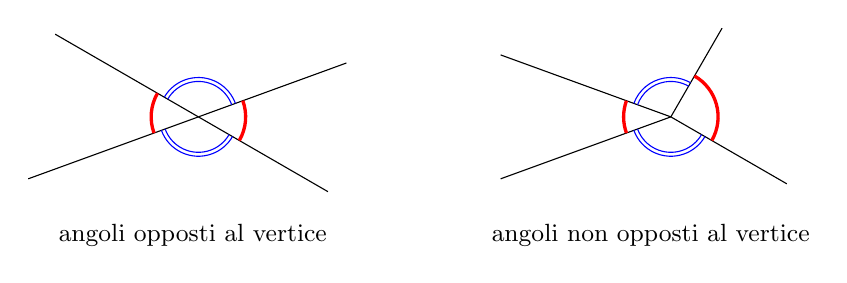
\begin{tikzpicture}
\pgfmathsetmacro{\myscale}{1};

\begin{scope}[scale={\myscale},font=\small]
\usetikzlibrary{calc}

\begin{scope}
\pgfmathsetmacro{\aalpha}{20};
\pgfmathsetmacro{\abeta}{150};
\pgfmathsetmacro{\agamma}{200};
\pgfmathsetmacro{\adelta}{330};

\coordinate (o) at (0,0);
\draw (o) -- ++({\aalpha}:2) coordinate (a);
\draw (o) -- ++({\abeta}:2.1) coordinate (b);
\draw (o) -- ++({\agamma}:2.3) coordinate (c);
\draw (o) -- ++({\adelta}:1.9) coordinate (d);

\draw[thin,blue] ([shift=({\abeta}:.45)]o) arc [radius=.45, start angle={\abeta}, end angle={\aalpha}];
\draw[thin,blue] ([shift=({\abeta}:.5)]o) arc [radius=.5, start angle={\abeta}, end angle={\aalpha}];
\draw[very thick, red] ([shift=({\agamma}:.6)]o) arc [radius =.6, start angle={\agamma}, end angle={\abeta}];
\draw[thin,blue] ([shift=({\agamma}:.45)]o) arc [radius=.45, start angle={\agamma}, end angle={\adelta}];
\draw[thin,blue] ([shift=({\agamma}:.5)]o) arc [radius=.5, start angle={\agamma}, end angle={\adelta}];
\draw[very thick, red] ([shift=({\adelta}:.6)]o) arc [radius =.6, start angle={\adelta}, end angle={360+\aalpha}];

\coordinate [label=0:angoli opposti al vertice] (l1) at (-1.9,-1.5);
\end{scope}


\pgfmathsetmacro{\myxshift}{6cm};
\begin{scope}[xshift={\myxshift}]
\pgfmathsetmacro{\aalpha}{60};
\pgfmathsetmacro{\abeta}{160};
\pgfmathsetmacro{\agamma}{200};
\pgfmathsetmacro{\adelta}{330};

\coordinate (o) at (0,0);
\draw (o) -- ++({\aalpha}:1.3) coordinate (a);
\draw (o) -- ++({\abeta}:2.3) coordinate (b);
\draw (o) -- ++({\agamma}:2.3) coordinate (c);
\draw (o) -- ++({\adelta}:1.7) coordinate (d);

\draw[thin,blue] ([shift=({\abeta}:.45)]o) arc [radius=.45, start angle={\abeta}, end angle={\aalpha}];
\draw[thin,blue] ([shift=({\abeta}:.5)]o) arc [radius=.5, start angle={\abeta}, end angle={\aalpha}];
\draw[very thick, red] ([shift=({\agamma}:.6)]o) arc [radius =.6, start angle={\agamma}, end angle={\abeta}];
\draw[thin,blue] ([shift=({\agamma}:.45)]o) arc [radius=.45, start angle={\agamma}, end angle={\adelta}];
\draw[thin,blue] ([shift=({\agamma}:.5)]o) arc [radius=.5, start angle={\agamma}, end angle={\adelta}];
\draw[very thick, red] ([shift=({\adelta}:.6)]o) arc [radius =.6, start angle={\adelta}, end angle={360+\aalpha}];

\coordinate [label=0:angoli non opposti al vertice] (l1) at (-2.4,-1.5);

\end{scope}

\end{scope}
\end{tikzpicture}

\caption{Gli angoli formati dalle semirette a sinistra sono opposti al vertice; gli angoli formati dalle semirette a destra non lo sono}\label{fig:1.24}
\end{figure}


\section{Confronto e operazioni tra segmenti e angoli}

\subsection{Premessa intuitiva}

Nel linguaggio comune usiamo la parola ``uguale'' con un significato generico, spesso per indicare due oggetti che si assomigliano: due macchine uguali, due orologi uguali,~\ldots{} In aritmetica e in algebra usiamo la parola ``uguale'' per indicare oggetti matematici perfettamente uguali. Per esempio, $2=2$, ogni numero infatti è uguale solo a se stesso. Scriviamo anche $3+2=5$, per dire che il numero che si ottiene dalla somma di 3 e 2 è proprio il numero 5. Nei polinomi si enuncia il principio di identità dei polinomi, in base al quale due polinomi sono uguali se si possono scrivere formalmente allo stesso modo.

In geometria, usiamo il termine ``uguale'' per indicare due figure coincidenti nella forma e nella posizione. In altre parole due figure sono \emph{uguali} solo se sono esattamente la stessa figura. Tuttavia, in geometria siamo interessati a studiare soprattutto figure che senza essere del tutto identiche hanno delle caratteristiche in comune. Vediamo prima degli esempi intuitivi e successivamente tratteremo lo stesso tema ma in modo formalmente corretto.

\begin{figure}[htb]
\centering% (c) 2014 Daniele Masini - d.masini.it@gmail.com
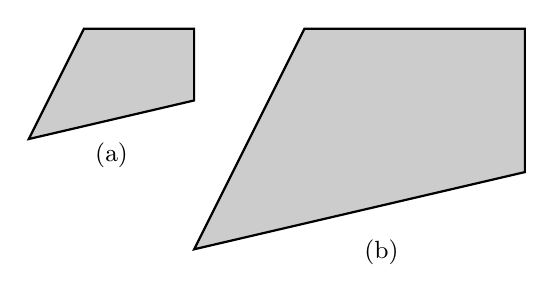
\begin{tikzpicture}[scale=.7,font=\small]
\usetikzlibrary{calc}

\begin{scope}
\coordinate (a) at (0,0);
\coordinate (b) at (1,2);
\coordinate (c) at (3,2);
\coordinate (d) at (3,0.7);
\draw[thick, fill={gray!40!white}] (a) -- (b) -- (c) -- (d) -- cycle;
\node at (1.5,-0.3) {(a)};
\end{scope}

\begin{scope}[xshift=3cm, yshift=-2cm, scale=2]
\coordinate (a) at (0,0);
\coordinate (b) at (1,2);
\coordinate (c) at (3,2);
\coordinate (d) at (3,0.7);
\draw[thick, fill={gray!40!white}] (a) -- (b) -- (c) -- (d) -- cycle;
\node at (1.7,-0.03) {(b)};
\end{scope}

\end{tikzpicture}
\qquad\qquad
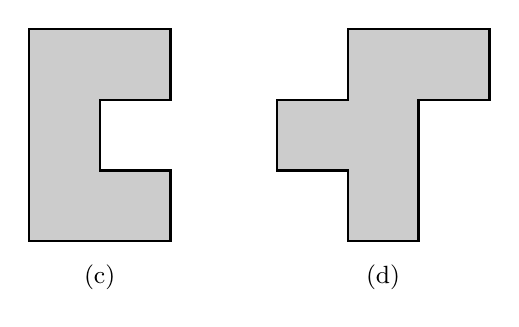
\begin{tikzpicture}[scale=.9,font=\small]
\usetikzlibrary{calc}

\begin{scope}
\coordinate (a) at (0,0);
\coordinate (b) at (2,0);
\coordinate (c) at (2,-1);
\coordinate (d) at (1,-1);
\coordinate (e) at (1,-2);
\coordinate (f) at (2,-2);
\coordinate (g) at (2,-3);
\coordinate (h) at (0,-3);
\draw[thick, fill={gray!40!white}] (a) -- (b) -- (c) -- (d) -- (e) -- (f) -- (g) -- (h) -- cycle;
\node at (1,-3.5) {(c)};
\end{scope}

\begin{scope}[xshift=3.5cm]
\coordinate (a) at (1,0);
\coordinate (b) at (3,0);
\coordinate (c) at (3,-1);
\coordinate (d) at (2,-1);
\coordinate (e) at (2,-3);
\coordinate (f) at (1,-3);
\coordinate (g) at (1,-2);
\coordinate (h) at (0,-2);
\coordinate (i) at (0,-1);
\coordinate (j) at (1,-1);
\draw[thick, fill={gray!40!white}] (a) -- (b) -- (c) -- (d) -- (e) -- (f) -- (g) -- (h) -- (i) -- (j) -- cycle;
\node at (1.5,-3.5) {(d)};
\end{scope}

\end{tikzpicture}

\end{figure}

Le figure (a) e (b), sopra riportate, hanno la stessa forma ma una è più grande dell'altra, la seconda infatti è stata ottenuta dalla prima raddoppiando la lunghezza di ogni lato: in geometria tali figure si dicono \emph{simili}.

Le figure (c) e (d), invece, non hanno la stessa forma e non si somigliano affatto, però le loro superfici hanno la stessa estensione, in quanto sono costituite dallo stesso numero di quadratini: in geometria tali figure si dicono \emph{equivalenti}.

\begin{figure}[htb]
\centering% Copyright (c) 2015 Daniele Masini - d.masini.it@gmail.com

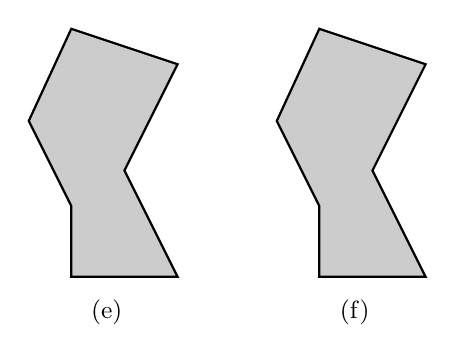
\begin{tikzpicture}[scale=.9,font=\small]
\usetikzlibrary{calc}

\begin{scope}
\coordinate (a) at (0,0);
\coordinate (b) at (1.5,-.5);
\coordinate (c) at (0.75,-2);
\coordinate (d) at (1.5,-3.5);
\coordinate (e) at (0,-3.5);
\coordinate (f) at (0,-2.5);
\coordinate (g) at (-0.6,-1.3);
\draw[thick, fill={gray!40!white}] (a) -- (b) -- (c) -- (d) -- (e) -- (f) -- (g) -- cycle;
\node at (0.5,-4) {(e)};
\end{scope}

\begin{scope}[xshift=3.5cm]
\coordinate (a) at (0,0);
\coordinate (b) at (1.5,-.5);
\coordinate (c) at (0.75,-2);
\coordinate (d) at (1.5,-3.5);
\coordinate (e) at (0,-3.5);
\coordinate (f) at (0,-2.5);
\coordinate (g) at (-0.6,-1.3);
\draw[thick, fill={gray!40!white}] (a) -- (b) -- (c) -- (d) -- (e) -- (f) -- (g) -- cycle;
\node at (0.5,-4) {(f)};
\end{scope}

\end{tikzpicture}
\qquad\qquad
% Copyright (c) 2015 Daniele Masini - d.masini.it@gmail.com

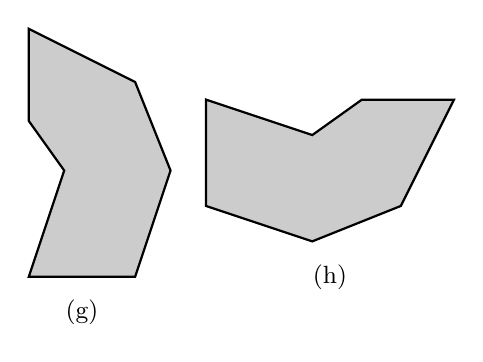
\begin{tikzpicture}[scale=.9,font=\small]
\usetikzlibrary{calc}

\begin{scope}
\coordinate (a) at (0,0);
\coordinate (b) at (1.5,-0.75);
\coordinate (c) at (2,-2);
\coordinate (d) at (1.5,-3.5);
\coordinate (e) at (0,-3.5);
\coordinate (f) at (0.5,-2);
\coordinate (g) at (0,-1.3);
\draw[thick, fill={gray!40!white}] (a) -- (b) -- (c) -- (d) -- (e) -- (f) -- (g) -- cycle;
\node at (0.75,-4) {(g)};
\end{scope}

\begin{scope}[xshift=3.5cm]
\begin{scope}[rotate=270,yshift=2.5cm, xshift=1cm]
\coordinate (a) at (0,0);
\coordinate (b) at (1.5,-0.75);
\coordinate (c) at (2,-2);
\coordinate (d) at (1.5,-3.5);
\coordinate (e) at (0,-3.5);
\coordinate (f) at (0.5,-2);
\coordinate (g) at (0,-1.3);
\draw[thick, fill={gray!40!white}] (a) -- (b) -- (c) -- (d) -- (e) -- (f) -- (g) -- cycle;
\end{scope}
\node at (0.75,-3.5) {(h)};
\end{scope}

\end{tikzpicture}

\end{figure}

Le figure (e) ed (f) hanno la stessa forma e le stesse dimensioni ma sono in posizioni differenti. \`E comunque possibile spostarle una sull'altra e farle coincidere. Usualmente le chiamiamo figure uguali, ma più precisamente in geometria tali figure si dicono \emph{congruenti}.

Le figure (g) e (h) hanno la stessa forma e le stesse dimensioni (per rendersene conto basta ruotare, per esempio, la seconda figura in senso antiorario e poi trascinarla sulla prima per sovrapporla). Anche queste figure sono dette uguali nel linguaggio comune, ma in geometria si dicono \emph{congruenti}.

Le figure (i) e (j), a pagina~\pageref{fig:figure_i_j}, hanno stessa forma e stesse dimensioni, tuttavia non si riesce a trasportare l'una sull'altra muovendole nel piano, né trascinandole, né ruotandole. Per farlo è necessario ribaltarne una facendola uscire dal piano, poiché le due figure sono una l'immagine speculare dell'altra. In geometria tali figure sono dette \emph{inversamente congruenti}.

\begin{figure}[htb]
\centering% (c) 2014 Daniele Masini - d.masini.it@gmail.com
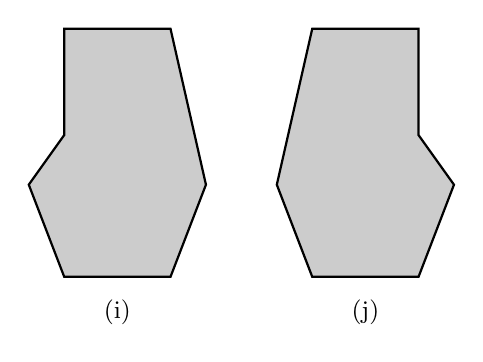
\begin{tikzpicture}[scale=.9,font=\small]
\usetikzlibrary{calc}

\begin{scope}
\coordinate (a) at (0,0);
\coordinate (b) at (1.5,0);
\coordinate (c) at (2,-2.2);
\coordinate (d) at (1.5,-3.5);
\coordinate (e) at (0,-3.5);
\coordinate (f) at (-0.5,-2.2);
\coordinate (g) at (0,-1.5);
\draw[thick, fill={gray!40!white}] (a) -- (b) -- (c) -- (d) -- (e) -- (f) -- (g) -- cycle;
\node at (0.75,-4) {(i)};
\end{scope}

\begin{scope}[xshift=5cm, xscale=-1]
\coordinate (a) at (0,0);
\coordinate (b) at (1.5,0);
\coordinate (c) at (2,-2.2);
\coordinate (d) at (1.5,-3.5);
\coordinate (e) at (0,-3.5);
\coordinate (f) at (-0.5,-2.2);
\coordinate (g) at (0,-1.5);
\draw[thick, fill={gray!40!white}] (a) -- (b) -- (c) -- (d) -- (e) -- (f) -- (g) -- cycle;
\node at (0.75,-4) {(j)};
\end{scope}

\end{tikzpicture}
\label{fig:figure_i_j}
\end{figure}

\osservazione Per ribaltare una figura occorre una dimensione in più rispetto a quelle della figura, precisamente se si tratta di due figure piane (che hanno due dimensioni: lunghezza e larghezza)  occorre avere la terza dimensione per effettuare un ribaltamento; se siamo su una retta (una sola dimensione: la lunghezza) occorre la seconda dimensione per ribaltare un segmento.

Per renderci conto di quanto accade con le figure solide, possiamo pensare ai palmi delle nostre mani che con buona approssimazione si possono considerare inversamente congruenti: esse possono essere giunte, ma non sovrapposte. Infatti non è possibile vedere le proprie mani sovrapposte, entrambe dal dorso o entrambe dal palmo, con le dita rivolte verso l'alto.

\subsection{La congruenza}

Secondo il punto di vista del matematico tedesco Felix Klein (1848-1925), la geometria è lo studio delle proprietà delle figure che sono invarianti rispetto a certe trasformazioni. Nello studio della geometria euclidea, quella che tratteremo in questo Tema, ci occupiamo delle proprietà delle figure geometriche invarianti rispetto ai movimenti rigidi, cioè rispetto a quei movimenti che conservano forma e dimensioni delle figure. Queste trasformazioni vengono anche dette \emph{isometrie} (si intuisce dalla radice etimologica che si parla di stessa misura): significa che viene stabilita una corrispondenza biunivoca tra i punti di due figure congruenti in modo da ``mantenere'' le distanze.

\begin{definizione}
Diciamo che due figure $F$ e $G$ sono \emph{congruenti} quando esiste un movimento rigido che le sovrappone perfettamente. In simboli $F\cong G$.
\end{definizione}

Nella Premessa a questo paragrafo abbiamo dato un'idea intuitiva e sperimentale del concetto di congruenza. Ma per esplicitarlo matematicamente dobbiamo utilizzare gli assiomi di congruenza di Hilbert che abbiamo enunciato nella sezione~\ref{sect:ass_Hilbert}. Ne riportiamo alcuni per comodità del lettore.

\begin{comment}

Assiomi di congruenza
	Assioma del trasporto di un segmento. Se A, B sono due punti di una retta a e A' è un punto sulla stessa retta o su un’altra retta a', si può sempre trovare un punto B' sulla retta a o su a’, da una data parte rispetto ad A', tale che il segmento AB sia congruente al segmento A'B'.
Questo assioma afferma che, fissato un punto A’ su una retta a’, è sempre possibile trasportare un qualunque segmento AB in modo che l’estremo A coincida con A’ e il segmento stia sulla retta a’.

	La relazione di congruenza tra segmenti è transitiva, cioè se A′B′ e A′′B′′ sono congruenti ad AB, allora A′B′  è congruente a A′′B′′.
La relazione di congruenza tra segmenti è allora un relazione di equivalenza, in quanto gode delle proprietà:
	riflessiva: ogni segmento è congruente a se stesso;
	simmetrica: se AB è congruente a A’B’ allora anche A’B’ è congruente ad AB;
	transitiva: se AB è congruente ad A’B’ e A’B’ è congruente ad A”B”, allora AB è congruente ad A”B”.

DEFINIZIONE. Si dice lunghezza di un segmento la classe di equivalenza dei segmenti congruenti tra di loro, cioè l’insieme di tutti i segmenti che sono congruenti tra di loro.
	Assioma del trasporto di un angolo. Dati un angolo AB ˆCed una semiretta B'C' , esistono e sono uniche due semirette B'D e B'E, tali che l'angolo D(B"'" ) ˆC"'" è congruente all'angolo AB ˆCe l'angolo E(B"'" ) ˆC"'" è congruente all'angolo AB ˆC.
Questo assioma ci garantisce che è sempre possibile trasportare un angolo  su una qualsiasi semiretta, facendo coincidere il vertice dell’angolo con l’origine della semiretta e un lato dell’angolo con la semiretta stessa.
	La relazione di congruenza tra angoli è transitiva, cioè se A"'" (B"'" ) ˆC"'"  eA"''" (B"''" ) ˆC"''"   sono congruenti ad AB ˆC, allora A"'" (B"'" ) ˆC"'"≡A"''" (B"''" ) ˆC"''" .

\end{comment}


%%%%%%%%%%%%%%%%%%%%%%%%%%%%%%%%%%%%%%%%%%%%%%%%%%%
\begin{comment}

Sappiamo che nel corso degli studi o nell'attività lavorativa possono presentarsi problemi di diversa natura: di tipo economico, scientifico, sociale; possono riguardare insiemi numerici o figure geometriche. La matematica ci può aiutare a risolvere i problemi quando essi possono essere tradotti in ``forma matematica'', quando cioè è possibile trascrivere in simboli le relazioni che intercorrono tra le grandezze presenti nel problema e quando si può costruire, tramite queste relazioni, un modello matematico che ci permetta di raggiungere la soluzione al quesito.

Affronteremo problemi di tipo algebrico o geometrico, che potranno essere formalizzati attraverso equazioni di secondo grado in una sola incognita.
Teniamo presente, prima di buttarci nella risoluzione del problema, alcuni passi che ci aiuteranno a costruire il modello matematico:
\begin{itemize*}
\item la lettura ``attenta'' del testo al fine di individuare l'ambiente del problema, le parole chiave, i dati e le informazioni implicite, l'obiettivo;
\item la scelta della grandezza incognita del problema, la descrizione dell'insieme in cui si ricerca il suo valore, le condizioni che devono essere soddisfatte dall'incognita;
\item la traduzione in ``forma matematica'' delle relazioni che intercorrono tra i dati e l'obiettivo, cioè l'individuazione del modello matematico (equazione risolvente).
\end{itemize*}
\begin{center}
 \input{./lbr/test/01test.pgf}
\end{center}

\begin{center}
 \input{./lbr/test/03test.pgf}
\end{center}

\begin{center}
 \input{./lbr/test/04test.pgf}
\end{center}

\begin{center}
 \input{./lbr/test/05test.pgf}
\end{center}

\begin{center}
 \input{./lbr/test/06test.pgf}
\end{center}
Dal punto di vista della struttura logica, gli \emph{Elementi} di Euclide sono organizzati a partire da cinque assiomi (nozioni comuni evidenti), cinque postulati (proposizioni che si richiede siano assunte come vere, senza dimostrazione) e 23 definizioni. L'opera di Euclide è rimasta nella nostra cultura l'unico punto di riferimento per lo studio della geometria, fino a quando, contestualmente allo studio dei fondamenti delle altre branche della matematica, i matematici cercarono di dare una base più rigorosa alla geometria di Euclide. Un'impostazione assiomatica più moderna venne data dal matematico tedesco David Hilbert nel libro \emph{Grundlagen der Geometrie} pubblicato nel 1899, nel quale la geometria veniva fondata su ben 21 assiomi.
\begin{center}
 \input{./lbr/test/07test.pgf}
\end{center}

\begin{center}
 \input{./lbr/test/08test.pgf}
\end{center}

\begin{problema}
Nel triangolo rettangolo $ABC$, rettangolo in $C$ l’ipotenusa supera il cateto maggiore $CB$ di $2\unit{m}$; la differenza tra i cateti è $23\unit{m}$. Determinare la misura del perimetro e l’area di $ABC$.
\end{problema}

\begin{multicols}{3}
\emph{Dati}

$\overline {AB} = \overline {CB} + 2$;

$\overline {CB} - \overline {AC} = 23$;

$A \widehat {C} B = \text{ retto}$.

\emph{Obiettivo}

$2 p$;

Area.

 \input{./lbr/chap03/fig004_tria.pgf}
\end{multicols}

\begin{soluzione}

Osserva che $2 p = \overline {AB} + \overline {BC} + \overline {AC}$ e $\Area =\frac{\overline {BC} \cdot \overline {AC}}{2}$.
Poni $\overline {BC} = x$; dai dati si ha $\overline {AB} = x + 2$ e $\overline{AC} = x - 23$ con
$\left\{\begin{array}{l} x > 0 \text{ essendo misura di un segmento} \\x >23 \text{ poiché } \overline {AC} \text{ deve essere positiva}
\end{array}\right.$.

Essendo il triangolo rettangolo, i lati sono legati dal teorema di Pitagora
quindi si deve verificare: $\overline {AB}^{2}= \overline {AC}^{2} + \overline {BC}^{2}\rightarrow ( x + 2 )^{2} = ( x - 23 )^{2} + x^{2}$. Sviluppando i calcoli si ottiene l'equazione risolvente di secondo grado, in forma canonica: $x^{2} - 50 x + 525 = 0 \text{ con } \Delta = 400$. L’equazione è determinata con il discriminante positivo, quindi esistono due soluzioni reali distinte: $x_{1} = 15 \vee x_{2} = 35$ entrambe positive. Ai fini del problema $x_{1} = 15$ non è accettabile, quindi il problema ha una sola soluzione e $\overline {BC} = 35$; $\overline {AB} = 37$; $\overline {AC} = 12$. Conclusione: $2 p = 35 + 37 + 12 = 84\unit{m}$; $ \Area = 210\unit{m^{2}}$.
\end{soluzione}

\begin{problema}
Un padre aveva $26$ anni alla nascita del figlio; moltiplicando le età attuali del padre e del figlio si trova il triplo del quadrato dell'età del figlio; calcolare le due età.
\end{problema}
Indichiamo con $p$ l'età attuale del padre e con $f$ l'età del figlio

\emph{Dati}: $p = f + 26;\; p \cdot f = 3 f^{2}$.
writer2latex102
\emph{Obiettivo}: $f,\; p$.

\begin{soluzione}
I dati permettono di impostare la relazione $(f + 26) \cdot f = 3 \cdot f^{2}$ che esprime il legame tra le età di oggi del padre e del figlio; siamo di
fronte ad un'equazione di secondo grado nell’incognita $f$. La soluzione dell’equazione deve essere espressa da un numero positivo poiché esprime l'età.
Risolviamo l'equazione $2 f^{2} - 26 f = 0$ le cui soluzioni sono $f_{1} = 0 \vee f_{2} = 13$. Per le condizioni poste la soluzione del problema è
$f = 13$. Quindi oggi il figlio ha $13$ anni e il padre $39$ anni.
\end{soluzione}

\begin{problema}
Il trapezio isoscele $ABCD$ è inscritto in una semicirconferenza di diametro $AB$ di misura $25\unit{cm}$; determina le misure dei lati del trapezio sapendo che il
perimetro è $62\unit{cm}$.
\end{problema}

\begin{multicols}{2}
\emph{Dati}

$\overline {AB} = 25$; $2 p = 62$;

$AB \parallel DC$; $\overline {AD} = \overline {CB}$.

\emph{Obiettivo}

$\overline {DC}$; $ \overline {CB}$.

 \input{./lbr/chap03/fig005_trap.pgf}
\end{multicols}

\begin{soluzione}
$\overline {AB} + \overline {DC} + 2 \overline {BC} = 62$; fissiamo come incognita la misura in cm di $BC$: $\overline {BC} = x$.
Determiniamo le condizioni sull’incognita: dovrà essere $x > 0$ poiché rappresenta la misura di un segmento e inoltre affinché esista
realmente il trapezio isoscele il punto $C$ non deve coincidere con il punto medio $E$ dell’arco $DC$ cioè $ CB<EB $, quindi $x < \dfrac{25}{2} \sqrt{2}$.

Tracciata l’altezza $CH (H \in AB)$ si ha $\overline {DC} = \overline {AB} - 2 \overline {HB}$ e per il 1° teorema di Euclide sul triangolo~$ACB$, rettangolo in
$C$, $\overline {HB}: \overline {CB} = \overline {CB} : \overline{AB}$; determiniamo quindi la misura di $HB$ in funzione dell’incognita fissata:
$\overline {HB} = \dfrac{x^{2}}{25}$ da cui $\overline {DC} = 25 - \dfrac{2 x^{2}}{25}$.

Costruiamo l’equazione risolvente: $25 + 2 x + 25 - \dfrac{2 x^{2}}{25} = 62 \rightarrow x^{2} - 25 x + 150 = 0$ che ha soluzioni $x_{1} = 10 \vee x_{2} = 15$, entrambe accettabili. Si hanno dunque due trapezi inscritti che risolvono il problema.
\begin{center}
 \input{./lbr/chap03/fig006_trap.pgf}
\end{center}
\end{soluzione}

\begin{problema}
Un capitale di $25000$ euro viene depositato in banca a un tasso di interesse annuo $c$. Gli interessi maturati durante il primo anno non vengono ritirati.
Nell'anno seguente si investono sia il capitale sia gli interessi maturati a un tasso di interesse annuo aumentato dello $0,5\%$. Alla fine dei due anni si ritira
la somma di $26291,10$ euro. Calcola i tassi di interesse praticati dalla banca.
\end{problema}
Assumiamo come incognita $c$ il tasso di interesse praticato il primo anno, espresso come numero decimale e
non in forma percentuale. Il tasso praticato nel secondo anno sarà $c+0,005$.

\begin{soluzione}
Alla fine del primo anno in banca rimane tra capitale e interessi \[25000 + 25000 \cdot c = 25000 ( 1 + c ).\] Nel secondo anno il tasso praticato è $c+0,005$ che va applicato alla somma $25000(1+c)$. Si~ottiene quindi l'equazione \[25000 ( 1 + c ) ( 1 + c + 0,005 ) = 26291,10.\]
Moltiplicando le parentesi tonde si ha $25000 ( 1,005 + c + 1,005 c + c^{2} ) = 26291,10$ e poi dividendo per $25000$ e ordinando otteniamo
$c^{2} + 2,005 c - 0,046644=0$ con soluzioni
\[c_{1,2}~=~\dfrac{- 2,005 \pm \sqrt{4,020025 + 0,186576}}{2} = \dfrac{-2,005 \pm 2,051}{2}\Rightarrow c_{1} = - 2,028 \vee c_{2} = 0,023.\]
La soluzione $c_1$ è negativa e non accettabile. La risposta al problema è $0,023$ cioè $2,3\%$ il primo anno e $2,8\%$ il secondo anno.
\end{soluzione}
\newpage
% (c) 2014 Daniele Masini - d.masini.it@gmail.com
\section{Esercizi}

\section{Esercizi riepilogativi}

\subsubsection*{\thechapter.1 - Primo teorema dell'angolo esterno}

\begin{esercizio}
\label{ese:3.1}
Vero o falso? In un triangolo:
\begin{enumeratea}
\item Per ogni lato c'è un solo angolo esterno\hfill\boxV\quad\boxF
\item Un angolo esterno è maggiore della somma degli angoli interni\hfill\boxV\quad\boxF
\item L'angolo esterno non può essere acuto\hfill\boxV\quad\boxF
\item L'angolo esterno è maggiore di ciascuno dei tre angoli interni\hfill\boxV\quad\boxF
\item L'angolo interno è minore di ciascuno degli angoli esterni non adiacenti\hfill\boxV\quad\boxF
\item L'angolo esterno è maggiore di ciascuno degli angoli interni ad esso non adiacenti\tab\tab\hfill\boxV\quad\boxF
\end{enumeratea}
\end{esercizio}

\begin{esercizio}
\label{ese:3.2}
Per ciascun vertice del triangolo nella figura~\ref{fig:ese3.2} disegna un angolo esterno.
\end{esercizio}

\begin{figure}[htb]
\centering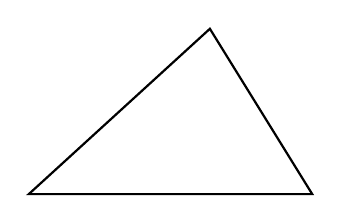
\begin{tikzpicture}[scale=1,font=\small]
\usetikzlibrary{calc, through, intersections}

\begin{scope}
\coordinate (a) at (0,0);
\coordinate (b) at (-2.3,-2.1);
\coordinate (c) at (1.3,-2.1);
%\draw[fill=gray!10] (a) -- (b) -- (c) -- cycle;

%\draw[thick] (a) node[above] {$A$} -- (b) node[left] {$B$} -- (c) node[right] {$C$} -- cycle;
\draw[thick] (a) -- (b) -- (c) -- cycle;

\end{scope}

\end{tikzpicture}

\caption{Esercizio~\ref{ese:3.2}}\label{fig:ese3.2}
\end{figure}

\begin{esercizio}
\label{ese:3.3}
Nel triangolo isoscele $ABC$ di base $AB$ prolunga il lato $CB$ fino a un punto $D$. Dimostra che: $A\widehat{B}D>A\widehat{C}B$, $C\widehat{B}A>A\widehat{D}B$, $C\widehat{A}B>B\widehat{A}D$, $C\widehat{A}B>B\widehat{D}A$.
\end{esercizio}

\begin{esercizio}
\label{ese:3.4}
Internamente a un triangolo $ABC$ prendi un punto $D$. Congiungi $D$ con $A$, con $B$ e con $C$. Il prolungamento di $AE$ incontra il lato $BC$ nel punto $E$. Dimostra che: $B\widehat{D}E>B\widehat{A}D$, $B\widehat{D}C>B\widehat{A}C$, $A\widehat{E}B>C\widehat{D}B$.
\end{esercizio}

\begin{esercizio}
\label{ese:3.5}
Nel triangolo $ABC$ traccia la bisettrice $AP$ dell'angolo in $A$. Dimostra che nel triangolo $APC$, l'angolo in $P$ è maggiore dell'angolo in $A$.
\end{esercizio}

\begin{esercizio}
\label{ese:3.6}
Dimostra che la somma di due angoli interni di un triangolo è minore di un angolo piatto. (Considera l'angolo esterno a uno dei due angoli).
\end{esercizio}

\begin{esercizio}
\label{ese:3.7}
Dimostra che un triangolo non può avere più di due angoli retti.
\end{esercizio}

\begin{esercizio}
\label{ese:3.8}
Dimostra che un triangolo non può avere due angoli ottusi.
\end{esercizio}

\begin{esercizio}
\label{ese:3.9}
Dimostrare che gli angoli alla base di un triangolo isoscele devono essere acuti.
\end{esercizio}

\subsubsection*{\thechapter.2 - Rette perpendicolari}

\begin{esercizio}
\label{ese:3.10}
Vero o falso?
\begin{enumeratea}
\item Dati un punto $P$ e una retta $r$ esiste sempre una retta perpendicolare a $r$ e passante per $P$\tab\hfill\boxV\quad\boxF
\item Dati un punto $P$ e una retta $r$ esistono infinite rette passanti per $P$ e perpendicolari a $r$\tab\hfill\boxV\quad\boxF
\item L'unicità della perpendicolare per un punto a una retta è un assioma\hfill\boxV\quad\boxF
\item L'unicità della parallela per un punto a una retta è un assioma\hfill\boxV\quad\boxF
\end{enumeratea}
\end{esercizio}

\begin{esercizio}
\label{ese:3.11}
Una retta $a$ è perpendicolare a una retta $b$, la quale a sua volta è perpendicolare a una terza retta $c$. Tra loro, le rette $a$ e $c$ sono:
\[\text{a) parallele;\qquad b) perpendicolari;\qquad c) né parallele né perpendicolari.}\]
\end{esercizio}

\begin{esercizio}
\label{ese:3.12}
Disegna le rette passanti per $P$ e perpendicolari alle altre rette presenti nella figura~\ref{fig:ese3.12}.
\end{esercizio}

\begin{figure}[htb]
\centering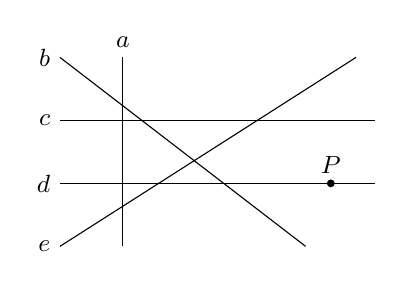
\begin{tikzpicture}[scale=0.8,font=\small]
\usetikzlibrary{calc, through, intersections}

\begin{scope}
\draw (0,0) coordinate (d1) node[left] {$d$} -- (5,0) coordinate (d2);
\draw (0,1) coordinate (c1) node[left] {$c$} -- (5,1) coordinate (c2);
\draw (1,-1) coordinate (a1) -- (1,2) coordinate (a2) node[above] {$a$};
\draw (0,2) coordinate (b1) node[left] {$b$} -- (3.9,-1) coordinate (c2);
\draw (0,-1) coordinate (e1) node[left] {$e$} -- (4.7,2) coordinate (e2);
\draw[fill] (4.3,0) circle (1.5pt) coordinate (p) node[above] {$P$};

%\draw[thick] (a) node[above] {$A$} -- (b) node[left] {$B$} -- (c) node[right] {$C$} -- cycle;

\end{scope}

\end{tikzpicture}

\caption{Esercizio~\ref{ese:3.12}}\label{fig:ese3.12}
\end{figure}

\begin{esercizio}
\label{ese:3.13}
Per ognuno dei punti di intersezione delle tre rette nella figura~\ref{fig:ese3.13} traccia la perpendicolare a ciascuna retta (aiutati con una squadretta).
\end{esercizio}

\begin{figure}[htb]
\centering% (c) 2014 Daniele Masini - d.masini.it@gmail.com
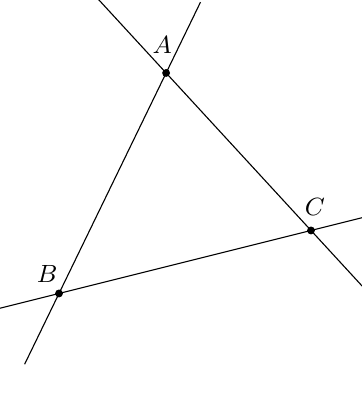
\begin{tikzpicture}[scale=0.8,font=\small, extended line/.style={shorten >=-#1,shorten <=-#1}, extended line/.default=1cm]
\usetikzlibrary{calc, through, intersections}

\begin{scope}
\coordinate (a) at (1.7,3.5);
\coordinate (b) at (0,0);
\coordinate (c) at (4,1);

\draw[extended line=1.5cm] (b) -- (c);
\draw[extended line] (a) -- (b);
\draw[extended line=1.3cm] (a) -- (c);

\draw[fill] (a) circle (1.5pt) node[shift={(-0.05,0.35)}] {$A$};
\draw[fill] (b) circle (1.5pt) node[shift={(-0.15,0.25)}] {$B$};
\draw[fill] (c) circle (1.5pt) node[shift={(0.05,0.3)}] {$C$};

%\path (a) circle (1);
%\path (b) circle (1);
%\path (c) circle (1.5);
\node at (0,-1) {};

%\draw[thick] (a) node[above] {$A$} -- (b) node[left] {$B$} -- (c) node[right] {$C$} -- cycle;

\end{scope}

\end{tikzpicture}

\caption{Esercizio~\ref{ese:3.13}}\label{fig:ese3.13}
\end{figure}

\begin{esercizio}
\label{ese:3.14}
Dimostra che le bisettrici di due angoli adiacenti sono perpendicolari.
\end{esercizio}

\subsubsection*{\thechapter.3 - Rette parallele}

\begin{esercizio}
\label{ese:3.15}
Vero o Falso?
\begin{enumeratea}
\item Due rette parallele tagliate da una trasversale formano quattro angoli alterni interni\tab\hfill\boxV\quad\boxF
\item Gli angoli corrispondenti sono a due a due interni o esterni\hfill\boxV\quad\boxF
\item Gli angoli interni si trovano da parti opposte rispetto alla trasversale\hfill\boxV\quad\boxF
\item Gli angoli esterni si trovano da parti opposte rispetto alla trasversale\hfill\boxV\quad\boxF
\item Due rette parallele possono anche coincidere\hfill\boxV\quad\boxF
\item La relazione di parallelismo tra rette è una relazione di equivalenza\hfill\boxV\quad\boxF
\item Due rette distinte hanno sempre un punto in comune\hfill\boxV\quad\boxF
\item Una retta che incontra due rette parallele forma angoli alterni interni supplementari\tab\hfill\boxV\quad\boxF
\item Per ogni retta è possibile tracciare una sola retta parallela\hfill\boxV\quad\boxF
\item Se due rette formano con una trasversale due angoli alterni interni allora sono parallele\tab\hfill\boxV\quad\boxF
\item Nel ragionamento per assurdo si nega l'ipotesi per dimostrare che la tesi è vera\tab\tab\hfill\boxV\quad\boxF
\item Ragionando per assurdo si nega la tesi e si ottenere una contraddizione con l'ipotesi\tab\hfill\boxV\quad\boxF
\end{enumeratea}
\end{esercizio}

\begin{esercizio}
\label{ese:3.16}
Nella figura~\ref{fig:ese3.16} disegna una parallela e una perpendicolare alla retta $r$ passanti per $P$ e una parallela e una perpendicolare a $s$ passanti per $Q$.
\end{esercizio}

\begin{figure}[htb]
\centering% Copyright (c) 2015 Daniele Masini - d.masini.it@gmail.com

\begin{tikzpicture}[scale=0.9,font=\small, extended line/.style={shorten >=-#1,shorten <=-#1}, extended line/.default=1cm]
\usetikzlibrary{calc, through, intersections}

\begin{scope}
\clip (-0.2,-0.1) rectangle (8.2,2.8);
\coordinate (p) at (3,0.3);
\coordinate (q) at (4.5,0.5);

\draw (0,0) node[above] {$r$} -- (5,3);
\draw (3,3) -- (8,0) node[above] {$s$};

\draw[fill] (p) circle (1.5pt) node[below] {$P$};
\draw[fill] (q) circle (1.5pt) node[below] {$Q$};

\end{scope}

\end{tikzpicture}

\caption{Esercizio~\ref{ese:3.16}}\label{fig:ese3.16}
\end{figure}

\begin{esercizio}
\label{ese:3.17}
Nella figura~\ref{fig:ese3.17} sono state tracciate due rette parallele e una trasversale. Indica con un arco gli angoli corrispondenti.
\end{esercizio}

\begin{figure}[htb]
\centering% Copyright (c) 2015 Daniele Masini - d.masini.it@gmail.com

\begin{tikzpicture}[scale=0.9,font=\small, extended line/.style={shorten >=-#1,shorten <=-#1}, extended line/.default=1cm]
\usetikzlibrary{calc, through, intersections}

\begin{scope}
\coordinate (p) at (3,0.2);
\coordinate (q) at (4.5,0.5);

\draw (0,0) -- (5,0.5);
\draw (0,1.2) -- (5,1.7);
\draw (1.5,-0.6) -- (3.5,2.4);

\end{scope}

\end{tikzpicture}

\caption{Esercizio~\ref{ese:3.17}}\label{fig:ese3.17}
\end{figure}

\begin{esercizio}
\label{ese:3.18}
Nella seguente figura sono state tracciate due rette parallele e una trasversale, sapendo che $\alpha=\frac{1}{3}\pi$, dove $\pi$ è l'angolo piatto, indica che frazione dell'angolo piatto sono gli altri angoli:\\
$\alpha=\frac{1}{3}\pi$\tab\tab $\beta = \ldots$\\
$\gamma=\ldots$\tab\tab $\delta = \ldots$\\
$\epsilon=\ldots$\tab\tab $\lambda = \ldots$\\
$\phi=\ldots$\tab\tab $\omega = \ldots$
\end{esercizio}

\begin{esercizio}
\label{ese:3.19}
Nella seguente figura $ABC$ è un triangolo isoscele, $IF$ è parallela a $BC$. Individua tutti gli angoli congruenti all'angolo $A\widehat{B}C$.
\end{esercizio}

\begin{esercizio}
\label{ese:3.20}
Completa ipotesi e tesi e metti in ordine le tre parti della dimostrazione:\\
In un triangolo $ABC$, isoscele su base $AB$, si prendano rispettivamente su $AC$ e $BC$ i punti $D$ ed $E$ equidistanti da $C$. Indicata con $S$ la proiezione di $D$ su $BC$ e con $U$ quella di $E$ su $AC$. Dimostrare che il segmento $US$ è parallelo ad $AB$.

\noindent Ipotesi: $AC\cong \ldots$, $D\in AC$, $E\in \ldots$, $S\in BC$, $DS\perp BC$, $U\in \ldots$, $EU\perp \ldots$.\tab Tesi: $US\parallel AB$.

Parte 1. I triangoli $CDS$ e $CEU$  hanno: l'angolo $\widehat{C}$ in comune, $CD$ \ldots{} $CE$ per \ldots\ldots{}, $D\widehat{S}C$ \ldots\ldots\ldots{} perché angoli \ldots\ldots{}, quindi tali triangoli sono congruenti per il \ldots\ldots\ldots{}, ne segue $CS \ldots CU$ e pertanto $C\widehat{U}S\cong \ldots$

Parte 2. Applicando il teorema sulla somma degli angoli interni ai triangoli $ABC$ e $CUS$, si ha che $C\widehat{U}S + C\widehat{S}U \ldots{} C\widehat{A}B + C\widehat{B}A$ perché supplementari dello stesso angolo $\widehat{C}$, ed essendo $\widehat{A}$ \dots{} $\widehat{B}$ perché \ldots\ldots\ldots{} ed essendo $C\widehat{U}S$ \ldots\ldots{} perché \ldots\ldots\ldots{}, risulta che $C\widehat{A}B$ \ldots{} $C\widehat{U}S$ perché \ldots\ldots\ldots{}

Parte 3. Gli angoli $C\widehat{A}B$ e $C\widehat{U}S$ (congruenti perché dimostrato) sono angoli \ldots\ldots rispetto alle rette $AB$ e $US$ tagliate dalla trasversale \ldots, quindi le rette $AB$ e $US$ sono parallele.
\end{esercizio}

\subsubsection*{Dimostra le seguenti affermazioni}
\begin{multicols}{2}

\begin{esercizio}
\label{ese:3.21}
Date due rette parallele tagliate da una trasversale, le bisettrici di due angoli corrispondenti (o alterni interni o alterni esterni) sono parallele.
\end{esercizio}

\begin{esercizio}
\label{ese:3.22}
Date due rette parallele tagliate da una trasversale, le bisettrici di due angoli coniugati interni (o coniugati esterni) sono perpendicolari.
\end{esercizio}

\begin{esercizio}
\label{ese:3.23}
Nel triangolo isoscele $ABC$ traccia una parallela alla base $AB$, che incontra i lati obliqui in $D$ ed $E$. Dimostra che anche $DCE$ è un triangolo isoscele.
\end{esercizio}

\begin{esercizio}
\label{ese:3.24}
Se due rette $r$ e $s$ sono incidenti allora lo sono anche due qualsiasi rette $u$ e $v$, con $u \parallel r$ e $v\parallel s$.
\end{esercizio}

\begin{esercizio}
\label{ese:3.25}
Sia $M$ il punto medio del segmento $AB$. Sia $r$ una retta che incontra $AB$ in $M$. Sulla retta $r$ da parti opposte rispetto a $M$ prendi due punti $C$ e $D$ in modo che $AC\parallel BD$. Dimostra che $AC\cong BD$. 
\end{esercizio}

\begin{esercizio}
\label{ese:3.26}
Dal vertice $C$ di un triangolo isoscele $ABC$ conduci la parallela alla base $AB$. Dimostra che tale parallela è bisettrice dell'angolo esterno in $C$ al triangolo.
\end{esercizio}

\begin{esercizio}
\label{ese:3.27}
Sia $ABC$ un triangolo isoscele di base $AB$. Sia $r$ la semiretta di origine $C$ bisettrice dell'angolo formato dal prolungamento di $BC$ e dal lato $AC$. Dimostra che la retta per $AB$ è parallela a $r$.
\end{esercizio}

\begin{esercizio}
\label{ese:3.28}
Dato il triangolo isoscele $ABC$ di base $AB$ e vertice $C$, prolunga la base $AB$ dalla parte di $A$ di un segmento $AD$. Sia $E$ un punto interno all'angolo $D\widehat{A}C$ in modo che $E\widehat{A}D\cong C\widehat{A}B$. Dimostra che $EA\parallel CB$.
\end{esercizio}

\begin{esercizio}
\label{ese:3.29}
Da ciascun vertice di un triangolo $ABC$ traccia la parallela al lato opposto. Detti $D$, $E$ ed $F$ i punti di intersezione delle parallele, dimostra che il triangolo $DEF$ ha gli angoli ordinatamente congruenti a quelli di $ABC$.
\end{esercizio}

\begin{esercizio}
\label{ese:3.30}
Sia $AD$ la bisettrice dell'angolo in $A$ del triangolo $ABC$. Dal punto $D$ traccia la parallela al lato $AB$, essa incontra il lato $AC$ in $E$. Dimostra che il triangolo $EDC$ ha gli angoli ordinatamente congruenti a quelli di $ABC$. Dimostra anche che $ADE$ è un triangolo isoscele.
\end{esercizio}

\begin{esercizio}
\label{ese:3.31}
In un triangolo $ABC$ rettangolo in $A$ traccia l'altezza $AH$ relativa all'ipotenusa. Dimostra che il triangolo $ABH$ ha gli angoli congruenti a quelli di $ABC$.
\end{esercizio}

\begin{esercizio}
\label{ese:3.32}
Sulla base $BC$ di un triangolo isoscele $ABC$ prendi un punto $D$ e traccia da esso la perpendicolare $p$ alla base. La suddetta perpendicolare incontra il lato $AB$ in $E$ e il lato $AC$ in $F$. Dimostra che il triangolo $AFE$ è isoscele.
\end{esercizio}

\begin{esercizio}
\label{ese:3.33}
In un triangolo $ABC$ traccia la bisettrice $AD$ dell'angolo in $A$. Da un punto $N$ del lato $AC$ traccia la parallela alla bisettrice $AD$, essa incontra che retta per $AB$ in $E$ e la retta per $BC$ in $F$. Dimostra che $AEN$ è un triangolo isoscele. Dimostra che $ADC$ e $NFC$ hanno angoli congruenti.
\end{esercizio}

\begin{esercizio}
\label{ese:3.34}
In un triangolo $ABC$ sia $E$ il punto di intersezione della bisettrice dell'angolo in $B$ con il lato $AC$. Sia $D$ un punto del lato $AB$ tale che $DE\cong DB$. Dimostra che $DE\parallel BC$.
\end{esercizio}

\begin{esercizio}
\label{ese:3.35}
In un triangolo $ABC$ traccia le bisettrici agli angoli nei vertici $B$ e $C$. Sia $D$ il punto di intersezione delle bisettrici. Da $D$ traccia la parallela al lato $BC$ e indica con $E$ ed $F$ i punti di intersezione di questa parallela con i lati rispettivamente $AB$ e $AC$. Dimostra che $FE\cong EB+FC$.
\end{esercizio}

\begin{esercizio}
\label{ese:3.36}
Dato il triangolo $ABC$ prolunga il lato $AB$ dalla parte di $A$ di un segmento $AD\cong AB$, prolunga poi il lato $AC$ dalla parte di $A$ di un segmento $AE\cong AC$. Dimostra che $DE\parallel BC$.
\end{esercizio}

\begin{esercizio}
\label{ese:3.37}
Sia $AM$ la mediana di un triangolo $ABC$. Si prolunghi $AM$ dalla parte di $M$ di un segmento $MD$ congruente ad $AM$. Dimostra che $CD$ è parallelo ad $AB$.
\end{esercizio}

\begin{esercizio}
\label{ese:3.38}
Due rette parallele tagliate da una trasversale formano otto angoli, uno di essi è $1/3$ dell'angolo retto. Determina le misure degli altri angoli.
\end{esercizio}

\begin{esercizio}
\label{ese:3.39}
Siano $\alpha$ e $\beta$ due angoli alterni interni formati da due rette parallele tagliate da una trasversale, dimostra che la bisettrice di $\alpha$ è parallela alla bisettrice di $\beta$.
\end{esercizio}

\begin{esercizio}
\label{ese:3.40}
Siano $\alpha$ e $\beta$ due angoli corrispondenti formati da due rette parallele tagliate da una trasversale, dimostra che la bisettrice di $\alpha$ è perpendicolare alla bisettrice di $\beta$.
\end{esercizio}

\begin{esercizio}
\label{ese:3.41}
Disegna due segmenti $AB$ e $CD$ disposti in modo che si incontrino nel loro punto medio comune $M$. Congiungi $A$ con $D$ e $B$ con $C$, dimostra che $AD$ è parallelo a $CB$.
\end{esercizio}

\begin{esercizio}
\label{ese:3.42}
Disegna un angolo acuto $a\widehat{O}b$ e la sua bisettrice $c$. Disegna su $c$ un punto $P$, disegna poi l'asse del segmento $OP$. Indica con $Q$ e $R$ i punti di intersezione dell'asse rispettivamente con la semiretta $a$ e la semiretta $b$. Dimostra che $OQ$ è parallelo a $RP$.
\end{esercizio}

\begin{esercizio}
\label{ese:3.43}
Disegna un angolo convesso $a\widehat{O}b$ e la sua bisettrice $c$. Disegna su $c$ un punto $P$, disegna poi le perpendicolari $PR$ e $PQ$ rispettivamente alle semirette $a$ e $b$. Dimostra che $c$ è asse del segmento $QR$.
\end{esercizio}

\begin{esercizio}
\label{ese:3.44}
Sia $ABC$ un triangolo equilatero. Traccia una parallela al lato $AB$ che incontra il lato $BC$ in $D$ e $AC$ in $E$. Dimostra che anche il triangolo $CDE$ è equilatero.
\end{esercizio}
\end{multicols}

\subsubsection*{\thechapter.4 - Somma degli angoli interni di un triangolo}

\begin{esercizio}
\label{ese:3.45}
Vero o Falso?
\begin{enumeratea}
\item La somma degli angoli interni di un triangolo è congruente a un angolo esterno\tab\tab\hfill\boxV\quad\boxF
\item La somma degli angoli interni di un quadrilatero è congruente a 3 angoli piatti\tab\tab\hfill\boxV\quad\boxF
\item La somma degli angoli esterni di un pentagono è congruente a 5 angoli piatti\hfill\boxV\quad\boxF
\item La somma degli angoli interni di un triangolo è congruente a due angoli retti\hfill\boxV\quad\boxF
\item Un triangolo isoscele non può avere un angolo ottuso\hfill\boxV\quad\boxF
\end{enumeratea}
\end{esercizio}

\subsubsection*{\thechapter.5 - Generalizzazione dei criteri di congruenza dei triangoli}

\begin{esercizio}
\label{ese:3.46}
Vero o Falso?
\begin{enumeratea}
\item Un triangolo rettangolo ha due angolo complementari\hfill\boxV\quad\boxF
\item Due triangoli rettangoli sono congruenti se hanno almeno un lato congruente\hfill\boxV\quad\boxF
\item Due triangoli rettangoli che hanno un cateto in comune sono congruenti\hfill\boxV\quad\boxF
\item Due triangoli rettangoli che hanno l'ipotenusa in comune sono congruenti\hfill\boxV\quad\boxF
\item Due triangoli rettangoli isosceli sono sempre congruenti\hfill\boxV\quad\boxF
\item Due triangoli rettangoli isosceli che hanno un lato in comune sono congruenti\hfill\boxV\quad\boxF
\item Gli angoli acuti di un triangolo rettangolo sono complementari\hfill\boxV\quad\boxF
\end{enumeratea}
\end{esercizio}

\begin{multicols}{2}

\subsubsection*{Dimostra le seguenti affermazioni}

\begin{esercizio}
\label{ese:3.47}
Dimostra che in triangolo rettangolo gli angoli diversi dall'angolo retto sono acuti.
\end{esercizio}

\begin{esercizio}
\label{ese:3.48}
Dimostra che non può esistere un triangolo rettangolo equilatero.
\end{esercizio}

\begin{esercizio}
\label{ese:3.49}
Due triangoli isosceli sono congruenti se hanno congruenti la base e l'angolo al vertice.
\end{esercizio}

\begin{esercizio}
\label{ese:3.50}
In un triangolo isoscele, le altezze relative ai lati congruenti sono congruenti. 
\end{esercizio}

\begin{esercizio}
\label{ese:3.51}
Due triangoli rettangoli sono congruenti se hanno congruenti un cateto e l'altezza relativa all'ipotenusa.
\end{esercizio}

\begin{esercizio}
\label{ese:3.52}
Due triangoli rettangoli sono congruenti se hanno congruenti un cateto e la mediana relativa ad esso.
\end{esercizio}

\begin{esercizio}
\label{ese:3.53}
Due triangoli rettangoli sono congruenti se hanno congruenti un angolo acuto e la sua bisettrice.
\end{esercizio}

\begin{esercizio}
\label{ese:3.54}
Se due triangoli hanno congruenti due coppie di lati e le mediane relative ai lati rimanenti, allora sono congruenti.
\end{esercizio}

\begin{esercizio}
\label{ese:3.55}
Dimostra che, in un triangolo isoscele, la bisettrice dell'angolo adiacente all'angolo al vertice è parallela alla base.
\end{esercizio}

\begin{esercizio}
\label{ese:3.56}
Dimostra che sono congruenti due triangoli isosceli che hanno gli angoli al vertice congruenti e congruenti le altezze relative a uno dei lati obliqui.
\end{esercizio}

\begin{esercizio}
\label{ese:3.57}
In un triangolo qualsiasi $ABC$ si prenda un qualsiasi punto del lato $AB$ e da esso si tracci la parallela $r$ alla bisettrice dell'angolo interno in $C$. Detto $P$ il punto di intersezione di $r$ con $AC$ e $Q$ il punto di intersezione di $r$ con $BC$, dimostra che $PC\cong QC$.
\end{esercizio}

\begin{esercizio}
\label{ese:3.58}
Sia $D$ il punto di intersezione delle bisettrici degli angoli in $A$ e in $B$ di un triangolo qualsiasi $ABC$. Per $D$ disegna la parallela al lato $AB$, indica con $E$ ed $F$ le intersezioni di questa parallela rispettivamente con il lati $AC$ e $BC$. Dimostra che $AF\cong AE+BF$.
\end{esercizio}

\begin{esercizio}
\label{ese:3.59}
Dimostra che, se per i vertici di un triangolo si conducono le parallele ai lati opposti, queste parallele determinano, assieme al triangolo dato, quattro triangoli congruenti.
\end{esercizio}

\begin{esercizio}
\label{ese:3.60}
Dimostra che in un triangolo isoscele la congiungente i punti medi dei lati congruenti è parallela alla base del triangolo.
\end{esercizio}

\begin{esercizio}
\label{ese:3.61}
Dimostrare che, in un triangolo rettangolo l'altezza relativa all'ipotenusa divide il triangolo in due triangoli rettangolo che hanno tra loro e col triangolo di partenza gli angoli ordinatamente congruenti.
\end{esercizio}

\begin{esercizio}
\label{ese:3.62}
Dato un triangolo $ABC$, si prolunghi il lato $CA$ dalla parte di $A$, si tracci la bisettrice dell'angolo interno di vertice $A$ e si conduca da $B$ la parallela a tale bisettrice, che incontri il prolungamento di $CA$ nel punto $D$. Dimostrare che il triangolo $ADB$ è isoscele.
\end{esercizio}

\begin{esercizio}
\label{ese:3.63}
Dato un angolo convesso $a\widehat{O}b$ traccia la sua bisettrice $c$. Per un punto $P$ della bisettrice traccia la perpendicolare alla bisettrice stessa. Chiama $A$ e $B$ i punto di intersezione della perpendicolare con i lati $a$ e $b$ dell'angolo convesso. Dimostra che $P$ è punto medio di $AB$.
\end{esercizio}

\begin{esercizio}
\label{ese:3.64}
Dato il triangolo isoscele $ABC$, di base $AB$, sul prolungamento dell'altezza relativa ad $AB$ prendi un punto $P$. Traccia la retta per $PA$ e per $PB$. Dimostra che l'angolo formato dalle rette $PA$ e $CA$ è congruente all'angolo formato dalle rette per $PB$ e $CB$.
\end{esercizio}

\begin{esercizio}
\label{ese:3.65}
Nel triangolo isoscele $ABC$ di vertice $A$ e lati congruenti $AB$ e $AC$, traccia le bisettrici degli angoli alla base. Sia $D$ il loro punto di intersezione. Dimostra che anche il triangolo $DBC$ è isoscele.
\end{esercizio}

\begin{esercizio}
\label{ese:3.66}
Dato un triangolo qualsiasi $ABC$ dimostra che la bisettrice dell'angolo interno in $A$ è perpendicolare alla bisettrice di uno degli angoli esterni in $A$.
\end{esercizio}

\begin{esercizio}
\label{ese:3.67}
Prolunga la mediana $M$ del triangolo $ABC$ di un segmento $MD$. Dimostra che se $AM\cong MD$ allora $BD$ è parallela a $CA$.
\end{esercizio}

\begin{esercizio}
\label{ese:3.68}
Sia $AM$ la mediana di un triangolo $ABC$. Dimostra che se $ABM$ è isoscele il triangolo $ABC$ è rettangolo e viceversa, se il triangolo $ABC$ è rettangolo in $A$ allora $ABM$ è isoscele.
\end{esercizio}

\begin{esercizio}
\label{ese:3.69}
Una retta $t$ incontra due rette $a$ e $b$ rispettivamente in $A$ e $B$. Dal punto medio $M$ di $AB$ traccia una retta che interseca $a$ e $b$ rispettivamente in $C$ e $D$. Dimostra che se $M$ è punto medio di $CD$ allora $a$ e $b$ sono parallele.
\end{esercizio}

\begin{esercizio}
\label{ese:3.70}
Nel triangolo isoscele $ABC$ prolunga la base $AB$ di un segmento $BD$ congruente a $BC$. Dimostra che l'angolo in $C$ esterno al triangolo $ADC$ è il triplo dell'angolo $ADC$.
\end{esercizio}

\begin{esercizio}
\label{ese:3.71}
Dato il triangolo $ABC$ traccia la retta $r$ perpendicolare ad $AB$ passante per $B$, la retta $s$ perpendicolare ad $AB$ passante per $A$, la retta $t$ perpendicolare ad $AC$ passante per $C$. Detti $D$ il punto di intersezione tra $r$ e $t$, $E$ il punto di intersezione tra $s$ e $t$, dimostra che $D\widehat{A}C+C\widehat{B}E+B\widehat{C}E$ è un angolo retto.
\end{esercizio}

\begin{esercizio}
\label{ese:3.72}
Nel triangolo $ABC$ traccia la media $CM$ e il suo prolungamento $MD$ a piacere. Da $A$ conduci la perpendicolare alla mediana che la incontra in $E$, da $B$ conduci un'altra perpendicolare alla mediana che la incontra in $F$. Dimostra che i triangoli $AEM$ e $BFM$ sono congruenti.
\end{esercizio}

\begin{esercizio}
\label{ese:3.73}
Sul prolungamento della base $AB$ di un triangolo isoscele individua un punto $D$ qualsiasi dalla parte di $B$. Traccia la perpendicolare per $D$ a questo prolungamento, essa incontra i lati obliqui del triangolo $AC$ e $BC$ rispettivamente in $E$ e in $F$. Dimostra che il triangolo $CEF$ è isoscele.
\end{esercizio}

\begin{esercizio}
\label{ese:3.74}
Siano $r$ e $s$ due rette incidenti in un punto $O$. Su $r$ prendi da parte opposta rispetto ad $O$ i punti $A$ e $B$ tali che $AO\cong OB$. Su $s$ prendi da parte opposta rispetto ad $O$ i punti $C$ e $D$ tali che $CO\cong OD$. Quale delle seguenti coppie di rette sono parallele? Dimostralo. ($CA\parallel BD$, $CB\parallel AD$)
\end{esercizio}

\begin{esercizio}
\label{ese:3.75}
Sia $ABC$ un triangolo acutangolo. Nel semipiano di origine $AB$ che non contiene $C$ individua un punto $D$ in modo che $B\widehat{A}D\cong C\widehat{B}A$. Dimostra che $CA\parallel AD$. Nell'ipotesi in cui $AD\cong CB$ dimostra che anche $AC\parallel BD$.
\end{esercizio}

\begin{esercizio}
\label{ese:3.76}
Calcola la misura degli angoli di un triangolo $ABC$ sapendo che l'angolo $A$ interno è $3/5$ dell'angolo esterno $A$ e che l'angolo $B$ è la metà di $A$.
\end{esercizio}

\begin{esercizio}[I Giochi di Archimede 2003]
\label{ese:3.77}
Sia data una stella a 5 punte inscritta in una circonferenza. Quanto vale la somma degli angoli con vertice nelle punte della stella? 
\end{esercizio}

\begin{esercizio}[I Giochi di Archimede 2003]
\label{ese:3.78}
Nella figura, quanto misura l'angolo $\alpha$?  
\end{esercizio}

\end{multicols}

\subsubsection*{\thechapter.6 - Disuguaglianze tra gli elementi di un triangolo}

\begin{esercizio}
\label{ese:3.79}
Vero Falso? 
\begin{enumeratea}
\item Esiste un triangolo i cui lati misurano 10~cm, 3~cm e 15~cm\hfill\boxV\quad\boxF
\item Un triangolo isoscele può essere ottusangolo\hfill\boxV\quad\boxF
\item Dati tre segmenti di cui almeno uno maggiore degli altri è sempre possibile costruire un triangolo che ha lati congruenti ai tre segmenti dati\hfill\boxV\quad\boxF
\item Dai tre segmenti di cui due uguali e uno maggiore degli altri due è sempre possibile costruire un triangolo isoscele che ha lati congruenti ai tre segmenti dati\hfill\boxV\quad\boxF
\item In un triangolo rettangolo l'ipotenusa è minore della somma dei due cateti\hfill\boxV\quad\boxF
\item Un triangolo di perimetro 100~cm non può avere un lato di 60~cm\hfill\boxV\quad\boxF
\item Un triangolo isoscele può essere ottusangolo\hfill\boxV\quad\boxF
\item In un triangolo l'angolo che si oppone al lato maggiore è acuto\hfill\boxV\quad\boxF
\item In un triangolo rettangolo i cateti sono sempre congruenti\hfill\boxV\quad\boxF
\item In un triangolo rettangolo l'ipotenusa può essere congruente ad un cateto\hfill\boxV\quad\boxF
\item Un triangolo può avere due lati disuguali e due angoli uguali\hfill\boxV\quad\boxF
\item In un triangolo rettangolo l'ipotenusa può essere congruente a un cateto\hfill\boxV\quad\boxF
\item Un triangolo può avere due angoli uguali e due lati disuguali\hfill\boxV\quad\boxF
\end{enumeratea}
\end{esercizio}

\begin{multicols}{2}

\subsubsection*{Dimostra le seguenti affermazioni}

\begin{esercizio}
\label{ese:3.80}
Sono dati due triangoli $ABC$ e $DEF$ di cui si sa che $\widehat{B}>\widehat{A}$, $\widehat{F}>\widehat{D}$, $BC\cong ED$. Dimostra che $AC>EF$.
\end{esercizio}

\begin{esercizio}
\label{ese:3.81}
Dimostra che in ogni triangolo rettangolo l'ipotenusa è maggiore di ciascun cateto.
\end{esercizio}

\begin{esercizio}
\label{ese:3.82}
Dimostra che in ogni triangolo rettangolo l'ipotenusa è maggiore della semisomma dei cateti.
\end{esercizio}

\begin{esercizio}
\label{ese:3.83}
In un triangolo ottusangolo il lato opposto all'angolo ottuso è maggiore di ciascuno degli altri due lati.
\end{esercizio}

\begin{esercizio}
\label{ese:3.84}
Dimostra che in un triangolo il doppio di un lato è minore del perimetro del triangolo. 
\end{esercizio}

\begin{esercizio}
\label{ese:3.85}
Dimostra che in un triangolo il doppio di una qualsiasi altezza è minore del perimetro del triangolo. 
\end{esercizio}

\begin{esercizio}
\label{ese:3.86}
Dimostra che in un poligono convesso una qualunque diagonale è minore del semiperimetro
\end{esercizio}

\begin{esercizio}
\label{ese:3.87}
Se in un triangolo due mediane sono congruenti, il triangolo è isoscele. 
\end{esercizio}

\begin{esercizio}
\label{ese:3.88}
Se due lati di un triangolo sono disuguali, la mediana uscente dal loro vertice comune forma con il lato opposto angoli disuguali ed è maggiore quello dalla parte del lato maggiore.
\end{esercizio}

\begin{esercizio}
\label{ese:3.89}
In un triangolo ogni lato è minore del semiperimetro.
\end{esercizio}

\begin{esercizio}
\label{ese:3.90}
In un triangolo l'altezza è minore della semisomma dei due lati che hanno un vertice in comune con essa.
\end{esercizio}

\begin{esercizio}
\label{ese:3.91}
In un triangolo, la mediana è minore della semisomma dei due lati che hanno un vertice in comune con essa.
\end{esercizio}

\begin{esercizio}
\label{ese:3.92}
In un triangolo $ABC$ traccia la bisettrice $BE$ dell'angolo in $B$. Dimostra che $AB>AE$. (Per la dimostrazione utilizza il teorema dell'angolo esterno).
\end{esercizio}

\begin{esercizio}
\label{ese:3.93}
Nel triangolo $ABC$ traccia la mediana $AM$. Dimostra che se $AC$ è maggiore di $AB$ allora l'angolo $A\widehat{M}C$ è maggiore dell'angolo $A\widehat{M}B$.
\end{esercizio}

\begin{esercizio}
\label{ese:3.94}
Nel triangolo $ABC$ prendi un punto $D$ interno al triangolo. Dimostra che il perimetro del triangolo $ADB$ è minore del perimetro del triangolo $ABC$. (Prolunga il lato $AD$ fino a incontrare il lato $BC$ in $E$. Ragionando opportunamente sui triangoli che si vengono a formare dimostra che $AD+DB<AC+CB$).
\end{esercizio}

\begin{esercizio}
\label{ese:3.95}
Esternamente al triangolo $ABC$ prendi un punto $D$. Congiungi $D$ con $A$, con $B$ e con $C$. Dimostra che il perimetro di $ABC$ è minore del doppio della somma delle distanze di $D$ dai tre vertici del triangolo.
\end{esercizio}

\begin{esercizio}
\label{ese:3.96}
Nel triangolo $ABC$ traccia la mediana $AM$ relativa al lato $BC$, dimostra che $AM$ è minore della semisomma degli altri due lati $AB$ e $BC$. (Prolunga la mediana di segmento congruente alla mediana stessa.)
\end{esercizio}

\begin{esercizio}
\label{ese:3.97}
In ogni triangolo, la somma delle mediane è minore del perimetro e maggiore del semiperimetro.
\end{esercizio}

\begin{esercizio}
\label{ese:3.98}
Dimostra che in un triangolo acutangolo, la somma delle altezze è minore del perimetro e maggiore del semiperimetro.
\end{esercizio}

\begin{esercizio}
\label{ese:3.99}
Dato un triangolo $ABC$ in cui $AB<AC$ traccia l'altezza $AH$ relativa alla base $BC$. Dimostra che l'angolo $H\widehat{A}C$ è maggiore dell'angolo $H\widehat{A}B$.
\end{esercizio}

\begin{esercizio}
\label{ese:3.100}
Dato il triangolo isoscele $ABC$ unisci il vertice $A$ con un punto $D$ della base $BC$. Dimostra che $AD$ è minore di ciascuno dei due lati congruenti, $AB$ e $AC$.
\end{esercizio}

\begin{esercizio}
\label{ese:3.101}
Dimostra in un poligono convesso, una qualunque diagonale è minore del semiperimetro.
\end{esercizio}

\begin{esercizio}
\label{ese:3.102}
In un triangolo $ABC$ si ha che $AB>AC$. Si tracci la bisettrice $AD$ dell'angolo in $A$. Si dimostri che $A\widehat{D}B>A\widehat{D}C$.
\end{esercizio}

\begin{esercizio}
\label{ese:3.103}
Due triangoli rettangoli hanno un cateto in comune e l'angolo opposto al cateto in comune è maggiore nel primo triangolo. Dimostra che l'ipotenusa del primo triangolo è minore di quella del secondo.
\end{esercizio}

\begin{esercizio}
\label{ese:3.104}
Dimostra che in ogni triangolo la somma dei tre lati è sempre maggiore del doppio di un lato.
\end{esercizio}

\begin{esercizio}
\label{ese:3.105}
Sia $AM$ la mediana di un triangolo generico $ABC$. Dimostra che se $AB>AC$ allora $A\widehat{M}C<A\widehat{M}B$.
\end{esercizio}

\begin{esercizio}
\label{ese:3.106}
Disegna un punto $D$ interno a un triangolo $ABC$ qualsiasi. Dimostra che $B\widehat{E}C>B\widehat{A}C$.
\end{esercizio}

\begin{esercizio}
\label{ese:3.107}
Sui lati $AB$, $BC$, $CA$ di un triangolo $ABC$ qualsiasi, scegli a caso tre punti, rispettivamente $D$, $E$ ed $F$. Dimostra che il perimetro di $ABC$ è maggiore del perimetro di $DEF$.
\end{esercizio}

\begin{esercizio}
\label{ese:3.108}
Un quadrilatero $ABCD$ si compone di un triangolo isoscele $ABC$ di base $BC$ e di un triangolo rettangolo isoscele $ACD$ con l'angolo retto in $C$. Dimostra che se l'angolo in $A$ del triangolo isoscele è acuto allora $BC<CD$, se l'angolo in $A$ del triangolo isoscele è ottuso risulta $CD<BC$.
\end{esercizio}

\end{multicols}

\begin{esercizio}[Prove invalsi 2004]
\label{ese:3.109}
Le rette $r$ ed $s$ sono tagliate dalla trasversale $t$. Quale delle seguenti condizioni permette di stabilire, per qualunque posizione di $t$, che $r$ ed $s$ sono parallele?\\
Gli angoli \ldots{}
\begin{enumeratea}
\item 1 e 5 sono supplementari;
\item 2 e 8 sono uguali;
\item 3 e 7 sono supplementari;
\item 4 e 7 sono uguali.
\end{enumeratea}
\end{esercizio}

\begin{esercizio}[Prove invalsi 2006]
\label{ese:3.110}
$r$ ed $s$ sono due rette parallele tagliate da una trasversale $t$. Quale tra le seguenti proposizioni è vera qualunque sia la posizione di $t$?
Gli angoli $\alpha$ e $\beta$ sono \ldots{}
\begin{enumeratea}
\item supplementari;
\item uguali;
\item complementari;
\item corrispondenti.
\end{enumeratea}
\end{esercizio}

\begin{esercizio}[Prove invalsi 2006]
\label{ese:3.111}
Per un triangolo ottusangolo qualsiasi, quale delle seguenti affermazioni è vera?
\begin{enumeratea}
\item La somma dei suoi due angoli più piccoli è minore dell'angolo più grande.
\item Il punto di incontro degli assi dei lati è certamente interno al triangolo.
\item Il triangolo è necessariamente isoscele.
\item Il triangolo può essere rettangolo.
\end{enumeratea}
\end{esercizio}

\begin{esercizio}[Prove invalsi 2004]
\label{ese:3.112}
In un triangolo, le misure dei lati sono $a$, $b$ e $c$, con $a = b < c$. Detti $\alpha$, $\beta$ e $\gamma$ gli angoli interni del triangolo, rispettivamente opposti ai lati $a$, $b$ e $c$, quale delle seguenti affermazioni è vera?
\begin{enumeratea}
\item $\alpha = \gamma$;
\item $\beta = \gamma$;
\item $\gamma > \alpha$;
\item $\alpha > \beta$.
\end{enumeratea}
\end{esercizio}

\begin{esercizio}[Prove invalsi 2010]
\label{ese:3.113}
Un triangolo ha un lato di 6~cm e uno di 10~cm. Quale tra le seguenti non può essere la misura della lunghezza del terzo lato?
\begin{enumeratea}
\item $\np{6,5}$~cm;
\item 10~cm;
\item $\np{15,5}$~cm;
\item 17~cm.
\end{enumeratea}
\end{esercizio}

\cleardoublepage
\end{comment}
% % % % % % % % % % % % % % % % % % % % % % % % % % % % % % % % % % % % % % % % % % % % % % % % % % % % % % % % % % % % %
